%%%%%%%%%%%%%%%%%%%%%%%%%%%%%%%%%%%%%%%%%
% Masters/Doctoral Thesis 
% LaTeX Template
% Version 2.5 (27/8/17)
%
% This template was downloaded from:
% http://www.LaTeXTemplates.com
%
% Version 2.x major modifications by:
% Vel (vel@latextemplates.com)
%
% This template is based on a template by:
% Steve Gunn (http://users.ecs.soton.ac.uk/srg/softwaretools/document/templates/)
% Sunil Patel (http://www.sunilpatel.co.uk/thesis-template/)
%
% Template license:
% CC BY-NC-SA 3.0 (http://creativecommons.org/licenses/by-nc-sa/3.0/)
%
%%%%%%%%%%%%%%%%%%%%%%%%%%%%%%%%%%%%%%%%%

%----------------------------------------------------------------------------------------
%	PACKAGES AND OTHER DOCUMENT CONFIGURATIONS

%----------------------------------------------------------------------------------------

\documentclass[
11pt, % The default document font size, options: 10pt, 11pt, 12pt
%oneside, % Two side (alternating margins) for binding by default, uncomment to switch to one side
english, % ngerman for German
singlespacing, % Single line spacing, alternatives: onehalfspacing or doublespacing
%draft, % Uncomment to enable draft mode (no pictures, no links, overfull hboxes indicated)
%nolistspacing, % If the document is onehalfspacing or doublespacing, uncomment this to set spacing in lists to single
%liststotoc, % Uncomment to add the list of figures/tables/etc to the table of contents
%toctotoc, % Uncomment to add the main table of contents to the table of contents
%parskip, % Uncomment to add space between paragraphs
%nohyperref, % Uncomment to not load the hyperref package
headsepline, % Uncomment to get a line under the header
%chapterinoneline, % Uncomment to place the chapter title next to the number on one line
%consistentlayout, % Uncomment to change the layout of the declaration, abstract and acknowledgements pages to match the default layout
]{MastersDoctoralThesis} % The class file specifying the document structure

\usepackage{unicode-math}

% ---------- Greek + English support (XeLaTeX) ----------
\usepackage{fontspec}
\usepackage{polyglossia}

\setdefaultlanguage{greek}
\setotherlanguage{english}

\setmainfont{DejaVu Serif}
\setsansfont{DejaVu Sans}
\setmonofont{DejaVu Sans Mono}
\newfontfamily\greekfonttt{DejaVu Sans Mono}

\usepackage[backend=biber,style=ieee]{biblatex} % Use the biber backend with the authoryear citation style (which resembles APA)

\addbibresource{example.bib} % The filename of the bibliography

\usepackage[autostyle=true]{csquotes} % Required to generate language-dependent quotes in the bibliography

%----------------------------------------------------------------------------------------
%	MARGIN SETTINGS
%----------------------------------------------------------------------------------------

\geometry{
	paper=a4paper, % Change to letterpaper for US letter
	inner=2.5cm, % Inner margin
	outer=3.8cm, % Outer margin
	bindingoffset=.5cm, % Binding offset
	top=1.5cm, % Top margin
	bottom=1.5cm, % Bottom margin
	%showframe, % Uncomment to show how the type block is set on the page
}

%----------------------------------------------------------------------------------------
%	THESIS INFORMATION
%----------------------------------------------------------------------------------------

\thesistitle{Αυτορρύθμιση Τεχνικών Εύρεσης Ανωμαλιών} % Your thesis title, this is used in the title and abstract, print it elsewhere with \ttitle
\supervisor{Prof. Αναστάσιος \textsc{Γούναρης}} % Your supervisor's name, this is used in the title page, print it elsewhere with \supname
\examiner{} % Your examiner's name, this is not currently used anywhere in the template, print it elsewhere with \examname
\degree{Προπτυχιακός Φοιτητής Πληροφορικής} % Your degree name, this is used in the title page and abstract, print it elsewhere with \degreename
\author{Ιωάννης \textsc{Σταθόπουλος}} % Your name, this is used in the title page and abstract, print it elsewhere with \authorname
\addresses{} % Your address, this is not currently used anywhere in the template, print it elsewhere with \addressname

\subject{Αυτορρύθμιση Τεχνικών Εύρεσης Ανωμαλιών} % Your subject area, this is not currently used anywhere in the template, print it elsewhere with \subjectname
\keywords{} % Keywords for your thesis, this is not currently used anywhere in the template, print it elsewhere with \keywordnames
\university{\href{https://www.auth.gr/}{Αριστοτέλειο Πανεπιστήμιο Θεσσαλονίκης}} % Your university's name and URL, this is used in the title page and abstract, print it elsewhere with \univname
\department{\href{https://www.auth.gr/faculty/sci/}{Σχολη Θετικών Επιστημών}} % Your department's name and URL, this is used in the title page and abstract, print it elsewhere with \deptname
\group{\href{http://researchgroup.university.com}{Research Group Name}} % Your research group's name and URL, this is used in the title page, print it elsewhere with \groupname
\faculty{\href{https://csd.auth.gr/}{Τμήμα Πληροφορικής}} % Your faculty's name and URL, this is used in the title page and abstract, print it elsewhere with \facname

\AtBeginDocument{
\hypersetup{pdftitle=\ttitle} % Set the PDF's title to your title
\hypersetup{pdfauthor=\authorname} % Set the PDF's author to your name
\hypersetup{pdfkeywords=\keywordnames} % Set the PDF's keywords to your keywords
}

\begin{document}

\frontmatter % Use roman page numbering style (i, ii, iii, iv...) for the pre-content pages

\pagestyle{plain} % Default to the plain heading style until the thesis style is called for the body content

%----------------------------------------------------------------------------------------
%	TITLE PAGE
%----------------------------------------------------------------------------------------

\begin{titlepage}
\begin{center}

\vspace*{.06\textheight}
{\scshape\LARGE \univname\par}\vspace{1.5cm} % University name
{\scshape\Large \deptname\par}\vspace{0.5cm} % Department name
{\scshape\large \facname\par}\vspace{0.5cm} % Faculty name
\textsc{\Large Πτυχιακή Εργασία}\\[0.5cm] % Thesis type


\HRule \\[0.4cm] % Horizontal line
{\huge \bfseries \ttitle\par}\vspace{0.4cm} % Thesis title
\HRule \\[1.5cm] % Horizontal line
 
\begin{minipage}[t]{0.4\textwidth}
\begin{flushleft} \large
\emph{Author:}\\
{\authorname} % Author name - remove the \href bracket to remove the link
\end{flushleft}
\end{minipage}
\begin{minipage}[t]{0.4\textwidth}
\begin{flushright} \large
\emph{Supervisor:} \\
{\supname} % Supervisor name - remove the \href bracket to remove the link  
\end{flushright}
\end{minipage}\\[3cm]

\begin{center}
	
\includegraphics[width=0.35\textwidth, height=0.9\textheight, keepaspectratio]{Figures/banner-vertical-300ppi.png}
	\label{fig:logo}
\end{center}

{\large \today}\\[4cm] % Date
%\includegraphics{Logo} % University/department logo - uncomment to place it
 
\vfill
\end{center}
\end{titlepage}

%----------------------------------------------------------------------------------------
%	DECLARATION PAGE
%----------------------------------------------------------------------------------------

\begin{declaration}
\addchaptertocentry{\authorshipname} % Add the declaration to the table of contents
\noindent Εγώ ο, \authorname, με πλήρη επίγνωση των συνεπειών του νόμου περί πνευματικών δικαιωμάτων, δηλώνω ότι η παρούσα πτυχιακή εργασία, καθώς και τα ηλεκτρονικά αρχεία και πηγαίοι κώδικες που αναπτύχθηκαν ή τροποποιήθκαν στο πλάισιο αυτής της εργασίας, αποτελεί αποκλειστικά προϊόν προσωπικής μου εργασίας, δεν προσβάλει κάθε μορφής δικαιώματα διανοητικής ιδιοκτησίας, προσωπικότητας και προσωπικών δεδομένων τρίτων, δεν περιέχει έργα/εισφορές τρίτων για τα οποία απαιτείται άδεια των δημιουργών/δικαιούχων και δεν είναι προϊόν μερικής ή ολικής αντιγραφής, οι πηγές δε που χρησιμοποιήθηκαν περιορίζονται στις βιβλιογραφικές αναφορές και μόνον, και πληρούν τους κανόνες της επιστημονικής παράθεσης. Τα σημεία όπου έχω χρησιμοποιήσει ιδέες, κείμενο, αρχεία ή/και πηγές άλλων συγγραφέων, αναφέρονται ευδιάκριτα στο κείμενο με την κατάλληλη παραπομπή και η σχετική αναφορά περιλαμβάνεται στο τμήμα βιβλιογραφικών αναφορών με πλήρη περιγραφή. Αναλαμβάνω πλήρως, ατομικά και προσωπικά, όλες τις νομικές και διοικητικές συνέπειες που δύναται να προκύψουν στην περίπτωση κατά την οποία αποδειχθεί, διαχρονικά, ότι η εργασία αυτή ή τμήμα της δεν μου ανήκει, διότι είναι προϊόν λογοκλοπής.
\vspace{5cm}

\end{declaration}

\cleardoublepage


%----------------------------------------------------------------------------------------
%	ABSTRACT PAGE
%----------------------------------------------------------------------------------------

\begin{abstract}
\addchaptertocentry{\abstractname} % Add the abstract to the table of contents
\indent Η ανίχνευση ανωμαλιών σε χρονοσειρές, είναι ένα πολύπλευρο πρόβλημα, το οποίο έχει κεντρίσει το ενδιαφέρον τόσο των εταιριών όσο και των ακαδημαϊκών, καθώς σχετίζεται με υψηλότερης ποιότητας εφαρμογές στην υγεία, σε χρηματοοϊκονομικά συστήματα, σε περιβαλλοντολογικές παρακολουθήσης καθώς και σε πολλούς άλλους τομείς.\newline \\
Η ανάγκη για την καλύτερη ανίχνευση ανωμαλιών, προοικονομεί ότι πρέπει να υπάρχει ένα σύστημα, το οποίο να μπορεί να αποφασίζει ποιός αλγόριθμος ή ποιό σύνολο αλγόριθμων είναι καταλληλότερο ανάλογα με το είδος της χρονοσειράς, ένα τρόπος ώστε να υπολογίζονται αυτόματα οι διάφορες υπερπαράμετροι του εκάστοτε αλγόριθμου, μία αμερόλπητη μετρική που να εφαρμόζεται σε όλα τα είδη των ανωμαλιών, καθώς επίσης και ένα σύστημα σημείου αναφοράς (benchmark), το οποίο θα αξιολογεί τις διάφορες τεχνικές ανίχνευσης ανωμαλιών που έχουν ή πρόκειται να προταθούν.\newline \\
Στα πλαίσια αυτής της πτυχιακής εργασίας, θα μελετήσουμε το σύστημα AutoTSAD \cite{schmidl2024autotsad}, ένα σύστημα το οποίο προτείνει μία αυτορυθμιζόμενη προσέγγιση για την ανίχνευση ανωμαλιώ σε χρονοσειρές, θα συγκρίνουμε τα αποτελέσματά ρων πιο αποτελεσματικών μεμονωμένων αλγορίθμων ανίχνευσης ανωμαλιών, χρησιμοποιώντας την μετρική VUS-PR \cite{paparrizos2022volume}, πάνω σε δεδομένα τα οποία έχουν συλλεχτεί από τους δημιουργούς του  TSB-UAD \cite{paparrizos2022tsb}.  
\end{abstract}

%----------------------------------------------------------------------------------------
%	ACKNOWLEDGEMENTS
%----------------------------------------------------------------------------------------

\begin{acknowledgements}
\addchaptertocentry{\acknowledgementname} % Add the acknowledgements to the table of contents
Ολοκληρώνοντας την πτυχιακή μου εργασία, θα ήθελα να ευχαριστήσω, αρχικά τον επιβλέποντα καθηγητή της εργαίας, κ. Αναστάσιο Γούναρη, προτίστως για την εμπιστοσύνη και την ευκαιρία που μου έδωσε να ασχοληθώ με το συγκεκριμένο θέμα, όπως επίσης και για την άμεση ανταπόκρισή και την συνεχή υποστήριξή του σε κάθε μου ερώτημα. \\
Επιπλέον ένα εγκάρδιο ευχαριστώ στην οικογένειά μου και κυρίως στην σύζυγό μου για την στήριξη που μου παρείχαν καθ' όλη τη διάρκεια αυτού του ταξιδιού, καθώς και να ζητήσω μία συγνώμη στις δύο μου κόρες, για όλες τις φορές που τους αρνήθηκα οποιαδήποτε δραστηριότητα μαζί τους, λόγω των ακαδημαϊκών υποχρεώσεων.\ldots
\end{acknowledgements}

%----------------------------------------------------------------------------------------
%	LIST OF CONTENTS/FIGURES/TABLES PAGES
%----------------------------------------------------------------------------------------

\tableofcontents % Prints the main table of contents

\listoffigures % Prints the list of figures

\listoftables % Prints the list of tables


%----------------------------------------------------------------------------------------
%	DEDICATION
%----------------------------------------------------------------------------------------

\dedicatory{For/Dedicated to/To my\ldots} 

%----------------------------------------------------------------------------------------
%	THESIS CONTENT - CHAPTERS
%----------------------------------------------------------------------------------------

\mainmatter % Begin numeric (1,2,3...) page numbering

\pagestyle{thesis} % Return the page headers back to the "thesis" style

% Include the chapters of the thesis as separate files from the Chapters folder
% Uncomment the lines as you write the chapters

% Chapter 1

\chapter{Εισαγωγή} % Main chapter title

\label{Chapter1} % For referencing the chapter elsewhere, use \ref{Chapter1} 

%----------------------------------------------------------------------------------------

% Define some commands to keep the formatting separated from the content 
\newcommand{\keyword}[1]{\textbf{#1}}
\newcommand{\tabhead}[1]{\textbf{#1}}
\newcommand{\code}[1]{\texttt{#1}}
\newcommand{\file}[1]{\texttt{\bfseries#1}}
\newcommand{\option}[1]{\texttt{\itshape#1}}

%----------------------------------------------------------------------------------------

\section{Το Πρόβλημα}

Η είσοδος στην καθημερινότητα μας, των συσκευών που συνδέονται στο Διαδύκτυο (IoT), έχει επηρεάσει αισθητά των όγκο των δεδομένων που συλλέγονται καθημερινά, καθώς και την ποικιλία τους. Το μεγαλύτερο ποσοστό αυτών των δεδομένων, είναι στην μορφή χρονοσειράς, δηλαδή μία ακολουθία από τιμές που έχουν καταγραφεί σε διαδοχικά χρονικά διαστήματα. Η ανίχνευση ανωμαλιών στις χρονοσειρές, είναι ένα πολύπλευρο πρόβλημα, το οποίο έχει κεντρίσει το ενδιαφέρον, τόσο των εταιριών αλλά και τον επιστημονικό κόσμο, καθώς σχετίζεται με υψηλότερης ποιότητας εφαρμογές στην υγεία, σε χρηματοοικονομικά συστήματα, σε περιβαλλοντολογικές παρακολουθήσεις, καθώς και σε πολλούς άλλους τομείς. Από την ανίχνευση ανωμαλιών μπορούμε να εξάγουμε πολύτιμες πληροφορίες, όπως π.χ. την ανίχνευση μία απάτης σε μία πιστωτική κάρτα, ή την ανίχνευση μίας σεισμικής δραστηριότητας, τον εντοπισμό ασυνήθιστης συμπεριφοράς ενός χρήστη σε ένα σύστημα κ.ο.κ

Τις τελευταίες δεκαετίες, έχουν προταθεί και αξιολογηθεί πληθόρα αλγορίθμων ανίχνευσης ανωμαλιών σε χρονοσειρές \cite{paparrizos2022tsb,gao2020ensemble,liu2008isolation,breunig2000lof,boniol2021sand,boniol2020automated,benecki2021detecting,boniol2021unsupervised,boniol2022theseus,boniol2021sand,yeh2016matrix,boniol2022series2graph,linardi2020matrix,yeh2018time,boniol2021sand_action}. Ωστόσο η επιλογή του κατάλληλου αλγορίθμου και η ρύθμιση των υπερπαραμέτρων του, είναι ένα πολυσύνθετο πρόβλημα, το οποίο εξαρτάται από το είδος της χρονοσειράς, των τύπο των ανωμαλιών, και απαιτεί πολύ χρόνο και υπολογιστικό κόστος.

Επίσης η έλλειψη ύπαρξης δεδομένων με ετικέτες για την εκπαίδευση των αλγορίθμων, μας οδηγεί σε μία μη-επιβλεπόμενη τεχνική για την ανίχνευση ανωμαλιών.

Τέλος, η έλλειψη ύπαρξης ενός καθολικού συστήματος σημείου αναφοράς (benchmark), το οποίο θα αξιολογεί τις διάφορες τεχνικές ανίχνευσης ανωμαλιών που έχουν ή πρόκειται να προταθούν, καθώς και μίας αμερόληπτης τεχνικής πέραν των παραδοσιακών, συνθέτουν ακόμα δύο προβλήματα προς εξερεύνηση.


%----------------------------------------------------------------------------------------

\section{Προτεινόμενες Λύσεις}

Τα τελευταία χρόνια (από το \date{2022} και μετά), έχουν προταθεί κάποια συστήματα, τα οποία έρχονται στοχεύουν στην επίλυση των προαναφερθέντων προβλημάτων.

\subsection{TSB-UAD Σύστημα σημείου αναφοράς (benchmark) για την ανίχνευση ανωμαλιών σε χρονοσειρές}

To 2022, προτάθηκε το \enquote{TSB: A Time Series Benchmark for Anomaly Detection} \cite{paparrizos2022tsb}, το οποίο αποτελείται από από μία συλλογή  αποτελούμενη από 13766 χρονοσειρές εκ των οποίων, οι 1980 προέρχονται από πραγματικά δεδομένα, οι 958 από τεχνητά δεδομένα, και 10828 συνθετικές χρονοσειρές κλιμακούμενης δυσκολίας.

Είναι ένα end-to-end benchmark, για μονοδιάστατες χρονοσειρές, το οποίο περιλαμβάνει μια ευρεία γκάμα τύπων ανωμαλιών. Προσπαθεί να παρέχει μία εννοιαία πλατφόρμα, σύγκρισης μεθόδων σε διαφορετικά ρεαλιστικά σενάρια, και να παρέχει ένα σύνολο από εργαλεία για την αξιολόγηση των αλγορίθμων ανίχνευσης ανωμαλιών σε χρονοσειρές.

\subsection{AutoTSAD: Ένα αυτοματοποιημένο σύστημα για την ανίχνευση ανωμαλιών σε χρονοσειρές}

To 2024, προτάθηκε το \enquote{AutoTSAD: Unsupervised Holistic Anomaly Detection for Time Series Data} \cite{schmidl2024autotsad} το οποίο είναι ένα μη-επιβλεπόμενο συνδιαστικό σύστημα ανίχνευσης ανωμαλιών σε μονοδιάστατες χρονοσειρές. Βασικά χαρακτηριστικά του έιναι ότι δεν απαιτεί την ύπαρξη ετικετών για την αξιολόγηση των αλγορίθμων, βασίζεται στον μηχανισμό Optuna \cite{akiba2019optuna} για την εύρεση των βέλτιστων υπερπαραμέτρων, και χρησιμοποιεί ένα ευρή φάσμα αλγορίθμων ανίχνευσης ανωμαλιών. Επίσης σε αντίθεση με άλλα συστήματα, το AutoTSAD επιστρέφει μία συνάθροιση βαθμολογιών, και όχι μία κατάταξη των αλγορίθμων. 

Τέλος μπορεί να λειτουργήσει και χωρίς την χρήση του μηχανισμού Optuna, παρά μόνο με προκαθορισμένες τιμές για τις υπερπαραμέτρους του κάθε αλγορίθμου, λόγω του τεράστιου απαιτούμενου χρόνου για την εύρεση των βέλτιστων υπερπαραμέτρων.

%----------------------------------------------------------------------------------------

\section{Σκοπός Πτυχιακής}
\label{purpose}

Σκοπός αυτής της πτυχιακής εργασίας, είναι η αξιολόγηση του AutoTSAD, το οποίο είναι ένα χρονικά απαιτητικό σύστημα, και να συγκριθέι η επίδοσή του, με μεμονωμένους αλγόριθμους, οι οποίοι έχουν καλή απόδοση ο καθένας σε διαφορετικά είδη τύπου ανωμαλιών, όπως ο MP \cite{linardi2020matrix}, ο IForest \cite{liu2008isolation}, ο POLY \cite{li1997poly} και NORMA \cite{mahin2024norma}, να παρουσιαστούν τα αποτελέσματα, και να αξιολογηθεί αν υπάρχει σοβαρή διαφορά η οποία να δικαιολογεί το χρονικό κόστος, πάντα με την χρήση αμερόληπτων τεχνικών, όπως η VUS-ROC\cite{paparrizos2022volume}.


%----------------------------------------------------------------------------------------


% Chapter 2

\chapter{Θεωρητικό Υπόβαθρο} % Main chapter title

\label{Chapter2} % For referencing the chapter elsewhere, use \ref{Chapter2} 
%----------------------------------------------------------------------------------------

% Define some commands to keep the formatting separated from the content 


%----------------------------------------------------------------------------------------

Σε αυτό το κεφάλαιο, θα δώσουμε κάποιους ορισμούς, για έννοιες που θα παρουσιαστούν αργότερα στα πλαίσια της εργασίας.


\section{Χρονοσειρές}

Χρονοσειρά ορίζεται ως μία ακολουθία από παρατηρήσεις, οι οποίες συλλέγονται ανά κανονικά/ακανόνιστα χρονικά διαστήματα, είναι διατεταγμένες σε χρονική σειρά, και λαμβάνονται από ιατρικά, οικονομικά, IoT, αισθητήρες, κ.ο.κ. Μπορεί να είναι μονοδιάστατες ή πολυδιάστατες, ανάλογα με τον αριθμό των μεταβλητών της κάθε μέτρησης. Στα πλαίσια της εργασίας θα ασχοληθούμε μόνο με μονοδιάστατες χρονοσειρές.

Συγκεκριμένα σύμφωνα με το \cite[Section 3.1]{schmidl2024autotsad}, ως μονοδιάστατες χρονοσειρές $T \in \mathrm{R}^n$ ορίζεται μία ακολουθία αληθινών μετρήσεων $T_i \in \mathrm{R}$, όπου $i \in |T|$ και $|T| = n$. Το μήκος της χρονοσειράς $T$ είναι $|T|$ ή $n$ και το i-οστό σημείο της ακολουθίας συμβολίζεται ως $T_i$.

%----------------------------------------------------------------------------------------

\section{Ανωμαλίες}

\emph{Ανωμαλίες} σε χρονοσειρές σύμφωνα με το \cite[Section 3.1]{paparrizos2022tsb}, ορίζονται ως σημεία, ή ακολουθίες σημείων, όπου αποκλίνουν σημαντικά από την κανονική συμπεριφορά της ακολουθίας, ή μίας υπακολουθίας της. Μπορεί να οφείλονται σε εσφαλμένες μετρήσεις ή σε πραγματικά ασυνήθιστα γεγονότα. Χωρίζονται σε τρεις κατηγορίες:
\begin{itemize}
    \item \emph{\bf{Point Anomalies}}: Αφορούν μεμονωμένα σημεία τα οποία διαφέρουν σημαντικά από τα υπόλοιπα σημεία της χρονοσειράς.
    \item \emph{\bf{Contextual Anomalies}}: Αφορούν σημεία, τα οποία μπορεί να είναι φυσιολογικά σε σχέση με τα υπόλοιπα σημεία της χρονοσειράς, αλλά να διαφέρουν σημαντικά δεδομένου ενός συγκεκριμένου πλαισίου.
    \item \emph{\bf{Collective anomalies}}: Αφορούν ακολουθίες σημείων, τα οποία δεν επαναλαμβάνουν ένα κανονικό, παρατηρήσιμο μοτίβο. Αξίζει να σημειωθεί, πως αν τα σημεία της υπακολουθίας παρατηρηθούν ως μεμωνομένα, μπορεί να ανιχνευτούν ως κανονικά από έναν αλγόριθμο ανίχνευσης ανωμαλιών.
\end{itemize}

\begin{figure}[h]
    \centering
    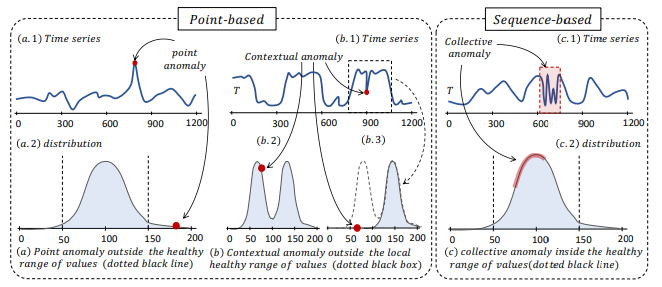
\includegraphics[width=1\linewidth]{Figures/anomalies_types.png}
    \caption{Τύποι ανωμαλιών σε χρονοσειρές (αναπαραγωγή από \cite{paparrizos2022tsb})}
    \label{figure:anomalies_types}
\end{figure}

Οι δημιουργοί του \emph{GutenTAG}\cite{10.14778/3554821.3554873} (βιβλιοθήκη για δημιουργία τεχνιτών χρονοσειρών με ή χωρίς ανωμαλίες), τις κατατάσουν στις εξής κατηγορίες:

\begin{itemize}
    \item \strong{Amplitude}: Αφορά στην αλλαγή του πλάτους του σήματος για κάποια χρονική περίοδο (Σχήμα \ref{figure:amplitude}).
    \begin{figure}[h]
    \centering
    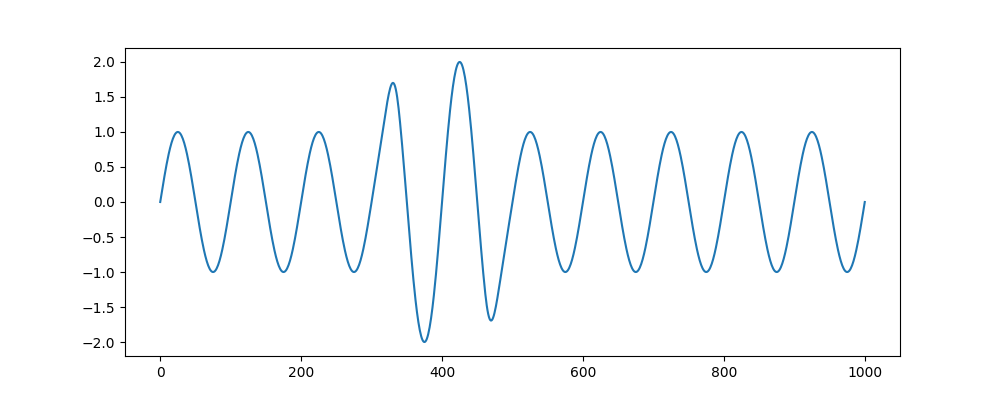
\includegraphics[width=1\linewidth]{Figures/gutenTAG_anomalies/amplitude.png}
    \caption{Amplitude anomaly (αναπαραγωγή από \cite{10.14778/3554821.3554873})}
    \label{figure:amplitude}
    \end{figure}
    \item  \strong{Extremum}: Αφορά την εμφάνιση μίας ακράια τιμής (spike) στο σήμα, το οποίο μπορεί να είναι είτε τοπικά μέγιστο-ελάχιστο, ή καθολικά μέγιστο-ελάχιστο (Σχήμα \ref{figure:extremum}).
    \begin{figure}[h]
    \centering
    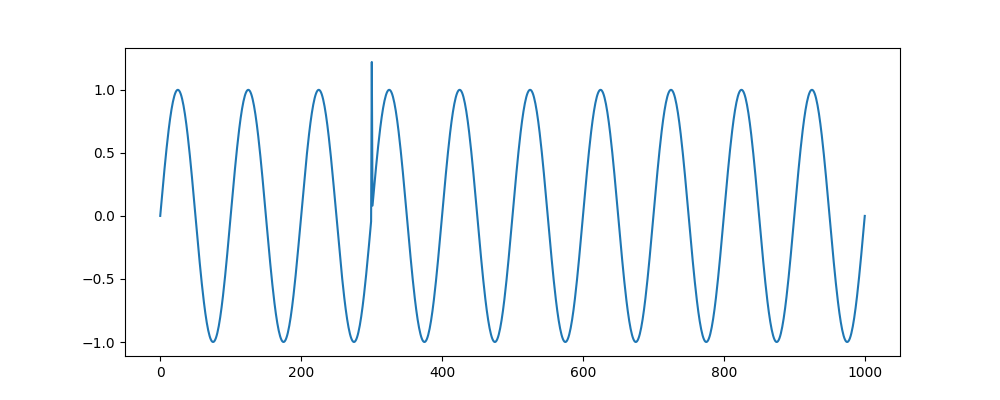
\includegraphics[width=1\linewidth]{Figures/gutenTAG_anomalies/extremum.png}
    \caption{Extremum anomaly (αναπαραγωγή από \cite{10.14778/3554821.3554873})}
    \label{figure:extremum}
    \end{figure}
    \item \strong{Συχνότητας}: Αφορά στην αλλαγή της συχνότητας σε μία χρονική περίοδο ενός σήματος (Σχήμα \ref{figure:frequency}).
    \begin{figure}[h]
    \centering
    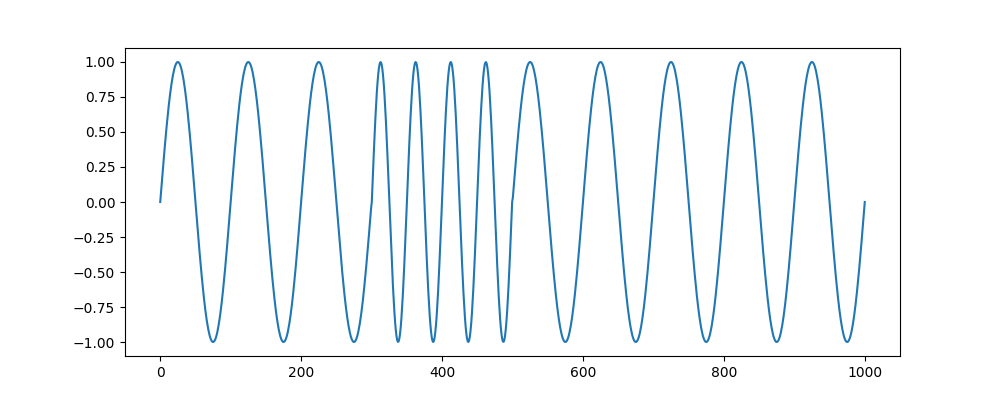
\includegraphics[width=1\linewidth]{Figures/gutenTAG_anomalies/frequency.png}
    \caption{Frequency anomaly (αναπαραγωγή από \cite{10.14778/3554821.3554873})}
    \label{figure:frequency}
    \end{figure}
    \item \strong{Mean}: Αφορά την κατακόρυφη μετατόπιση της χρονοσειράς κατά μία σταθερή τιμή για το διάστημα της ανωμαλίας (Σχήμα \ref{figure:mean}).
    \begin{figure}[h]
    \centering
    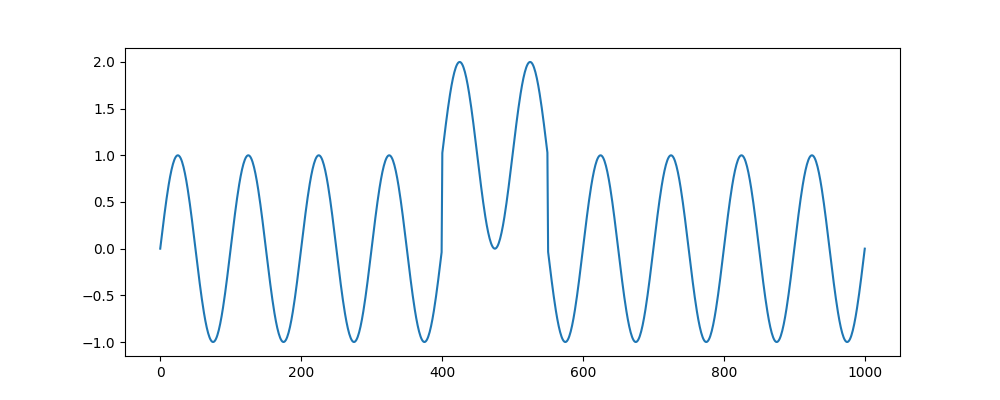
\includegraphics[width=1\linewidth]{Figures/gutenTAG_anomalies/mean.png}
    \caption{Mean anomaly (αναπαραγωγή από \cite{10.14778/3554821.3554873})}
    \label{figure:mean}
    \end{figure}
    \item \strong{Pattern}: Αφορά στην αλλαγή του επαναλαμβανόμενου μοτίβου της χρονοσειράς (π.χ. ένα ημιτονοειδές σήμα θα μπορούσε να παραμορφωθεί για το διάστημα της ανωμαλίας) (Σχήμα \ref{figure:pattern-ecg} και \ref{figure:pattern-shift}).
    \begin{figure}[h]
    \centering
    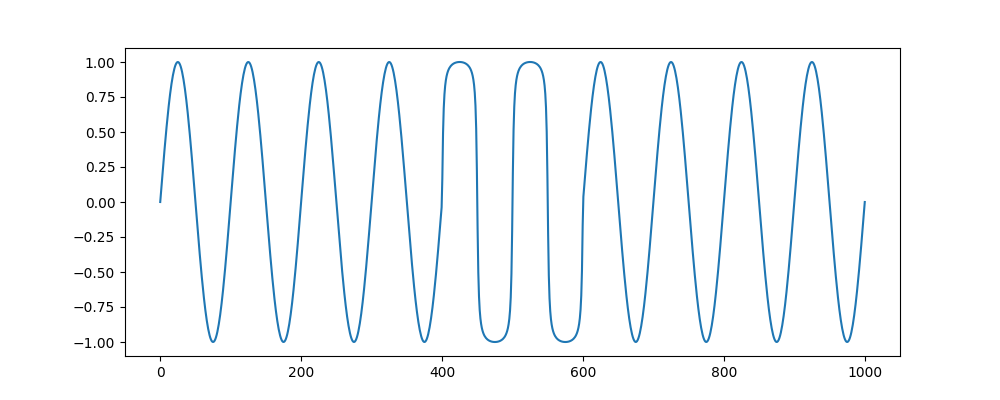
\includegraphics[width=1\linewidth]{Figures/gutenTAG_anomalies/pattern-sine.png}
    \caption{Pattern-sine anomaly (αναπαραγωγή από \cite{10.14778/3554821.3554873})}
    \label{pattern-sine}
    \end{figure}
    \begin{figure}[h]
    \centering
    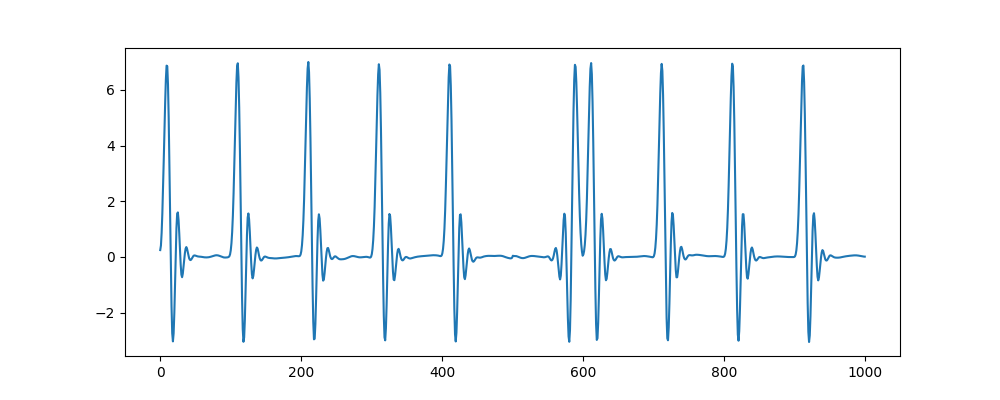
\includegraphics[width=1\linewidth]{Figures/gutenTAG_anomalies/pattern-ecg.png}
    \caption{Pattern-ecg anomaly (αναπαραγωγή από \cite{10.14778/3554821.3554873})}
    \label{figure:pattern-ecg}
    \end{figure}
    \item  \strong{Pattern Shift}: Αφορά την χρονική μετατόπιση του μοτίβου της χρονοσειράς (Σχήμα \ref{figure:pattern-shift}). 
    \begin{figure}[h]
    \centering
    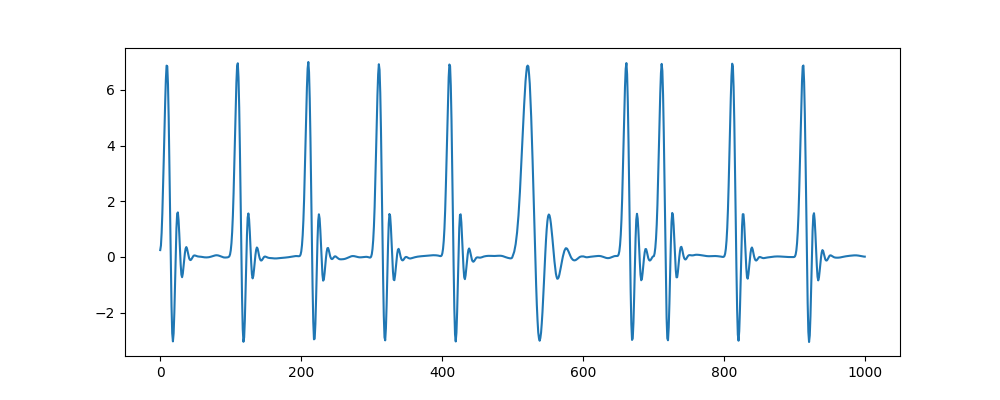
\includegraphics[width=1\linewidth]{Figures/gutenTAG_anomalies/pattern-shift.png}
    \caption{Pattern-shift anomaly (αναπαραγωγή από \cite{10.14778/3554821.3554873})}
    \label{figure:pattern-shift}
    \end{figure}
    \item \strong{Platform}: Για κάποιο χρονικά διάστημα, η χρονοσειρά "παγώνει" και έπειτα συνεχίζει κανονικά (π.χ. θα μπορούσαμε να το προσομοιάσουμε με την στιγμή που η καρδιά ενός ασθενή σταματάει να δουλεύει για κάποια δευτερολέπτα, ο ασθενής επαναφέρεται και η καρδιά δουλεύει πάλι κανονικά) (Σχήμα \ref{figure:platform}).
    \begin{figure}[h]
    \centering
    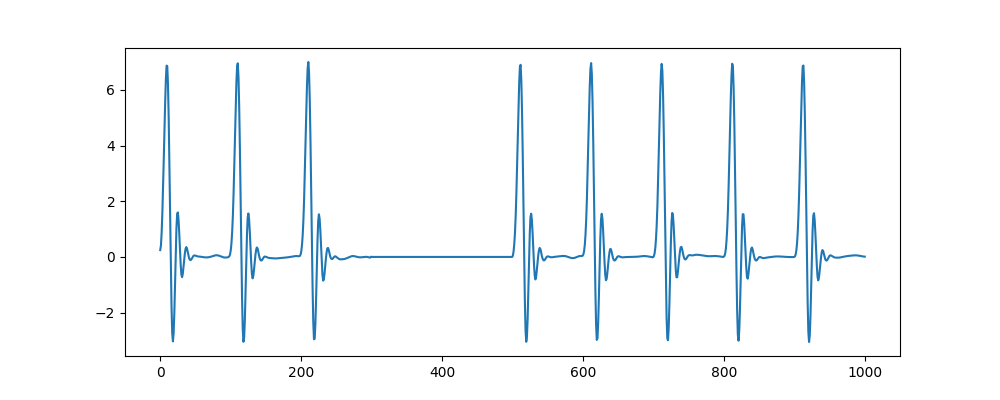
\includegraphics[width=1\linewidth]{Figures/gutenTAG_anomalies/platform.png}
    \caption{Platform anomaly (αναπαραγωγή από \cite{10.14778/3554821.3554873})}
    \label{figure:platform}
    \end{figure}
    \item \strong{Trend}: Αφορά σε μία αυξανόμενη ή μειούμενη τάση στην χρονοσειρά (Σχήμα \ref{figure:trend}).
    \begin{figure}[h]
    \centering
    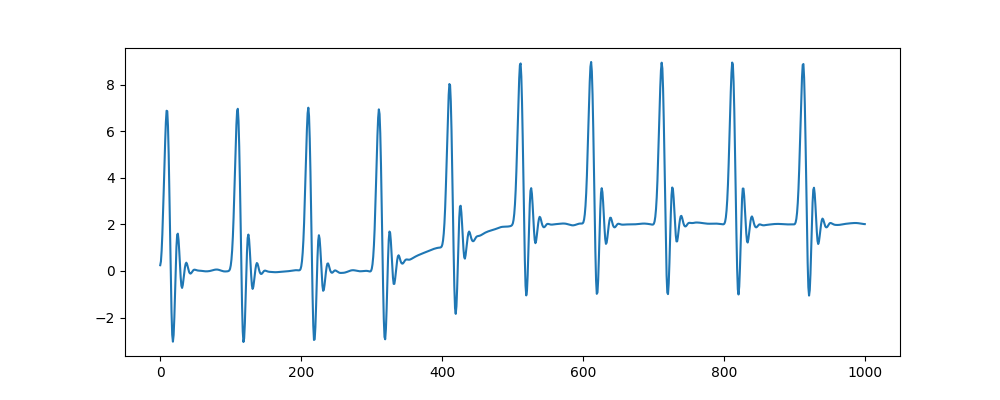
\includegraphics[width=1\linewidth]{Figures/gutenTAG_anomalies/trend.png}
    \caption{Trend anomaly (αναπαραγωγή από \cite{10.14778/3554821.3554873})}
    \label{figure:trend}
    \end{figure}
    \item \strong{Variance}: Αφορά στην μεταβολή του επίπεδου θορύβου για μία χρονική περίοδο της χρονοσειράς (Σχήμα \ref{figure:variance}).
    \begin{figure}[h]
    \centering
    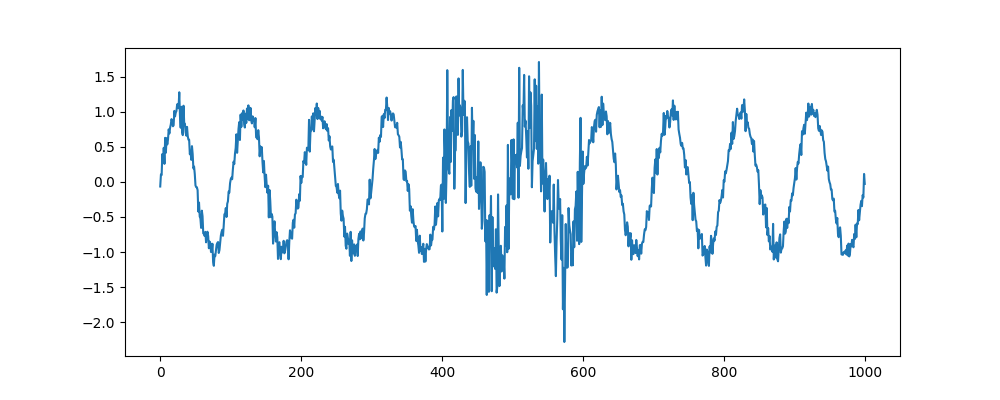
\includegraphics[width=1\linewidth]{Figures/gutenTAG_anomalies/variance.png}
    \caption{Variance anomaly (αναπαραγωγή από \cite{10.14778/3554821.3554873})}
    \label{figure:variance}
    \end{figure}
    \item \strong{Mode Correlation}: Αφορά στην αλλαγή της συμπεριφοράς μίας υπακολουθίας για το διάστημα που κρατάει η ανωμαλία (Σχήμα \ref{figure:mode-correlation}).
    \begin{figure}[h]
    \centering
    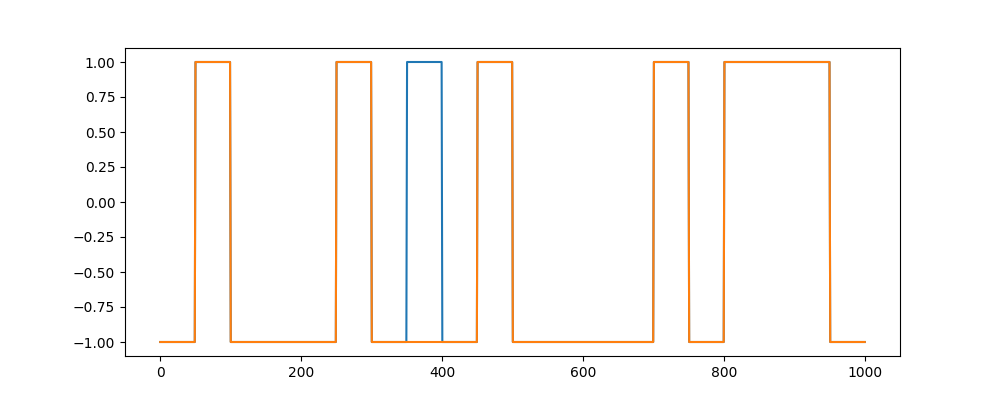
\includegraphics[width=1\linewidth]{Figures/gutenTAG_anomalies/mode-correlation.png}
    \caption{Mode correlation anomaly (αναπαραγωγή από \cite{10.14778/3554821.3554873})}
    \label{figure:mode-correlation}
    \end{figure}
\end{itemize}

Είναι πολύ πιθανό, σε χρονοσειρές πραγματικών δεδομένων, να παρατηρηθούν παραπάνω από ένας τύπος ανωμαλιών, ή ακόμα και συνδυασμοί αυτών. Τέτοια παραδείματα φαίνονται στο \ref{figure:anomalies_combined}. Στην (d.1) για παράδειγμα, μπορούμε να παρατηρήσουμε ένα \emph{point anomaly}, το \verb|A2| και ένα \emph{collective anomaly}, την υπακολουθία \verb|A1|. 

\begin{figure}[h]
    \centering
    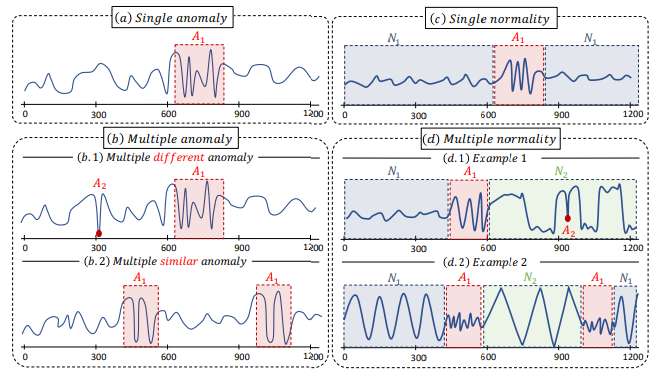
\includegraphics[width=0.7\linewidth]{Figures/anomalies_combined.png}
    \caption{Χρονοσειρές με διαφορετικούς τύπους ανωμαλιών (αναπαραγωγή από \cite{paparrizos2022tsb})}
    \label{figure:anomalies_combined}
\end{figure}



\section{Μεμονωμένοι Αλγόριθμοι Σύγκρισης}

Σε αυτό το σημείο, θα κάνουμε μία σύντομη αναφορά στους αλγορίθμους που αναφέρθηκαν στο \ref{purpose} και θα χρησιμοποιηθούν στην εργασία. Θα αναφερθεί ο τρόπος λειτουργίας τους, τα πλεονεκτήματα και τα μειονεκτήματά τους, πώς συνδέονται με την ανίχνευση ανωμαλιών, και πως οι υπερπαράμετροί τους επηρεάζουν την απόδοσή τους.

\subsection{Isolation Forest}
Οι περισσότεροι αλγόριθμοι ανίχνευσης ανωμαλιών, δημιουργούν ένα μοτίβο κανονικών δεδομένων και έπειτα, τα σημεία τα οποία αποκλίνουν από αυτό το μοτίβο, τα χαρακτηρίζουν ως ανωμαλίες. Αυτή η τεχνική έχει 2 αδυναμίες.
\begin{itemize}
    \item Πρώτον, ο αλγόριθμος είναι βελτιστοποιημένος ώστε να βρίσκει κανονικές συμπεριφορές, και όχι ανωμαλίες, οπότε μπορεί να μην είναι τόσο αποτελεσματικός στην ανίχνευση ανωμαλιών.
    \item Δεύτερον, οι περισσότερες μεθόδοι περιορίζονται σε χαμηλές διαστάσεις δεδομένων, ή και μικρό όγκο δεδομένων, λόγο της υπολογιστικής πολυπλοκότητας που απαιτείται.
\end{itemize}
Αντιθέτως, ο \emph{iForest} ακολουθεί μία διαφορετική τακτική, στοχοποιεί τις ανωμαλίες, αξιοποιώντας 2 βασικές ιδιότητες των ανωμαλιών.
\begin{itemize}
    \item Πρώτον, οι ανωμαλίες αποτελούν την μειονότητα των δεδομένων.
    \item Δεύτερον, έχουν χαρακτηριστικά τα οποία διαφέρουν πολύ από τα κανονικά δεδομένα.
\end{itemize}
Επειδή οι ανωμαλίες απομονώνονται ευκολότερα από τα κανονικά δεδομένα, βρίσκονται πιο κοντά  στην ρίζα του δένδρου. Στο
σχήμα \ref{figure:iForest1}(a), παρατηρούμε πως το σημείο $x_i$ απαιτεί περισσότερες διχοτομήσεις για να απομονωθεί, σε αντίθεση με το σημείο $x_0$, όπως φαίνεται στο \ref{figure:iForest1}(b). Επίσης στο σχήμα \ref{figure:iForest1}(c), παρατηρούμε πως η μέση απόσταση των σημείων $x_0$ και $x_i$ από την ρίζα του δένδρου, σταθεροποιείται, με μικρό αριθμό δένδρων ($n\approx10$), γεγονός που αποδυκνύει πως ο \emph{iForest} δεν απαιτεί μεγάλο αριθμό δέδρων για να συγκλίνει σε ένα καλό αποτέλεσμα.
\begin{figure}
    \centering
    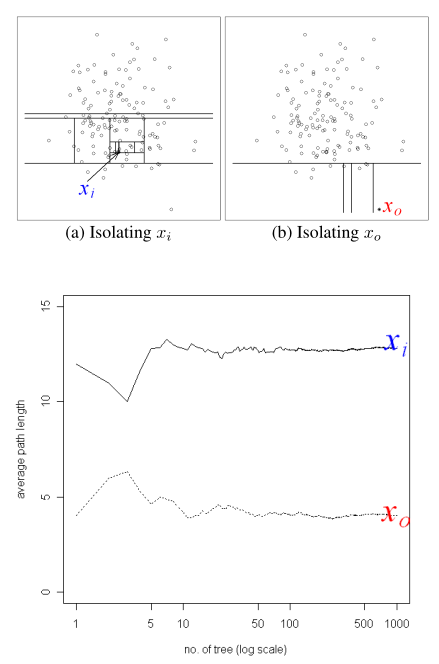
\includegraphics[width=1\linewidth]{Figures/iForest1.png}
    \caption{(a) Απομόνωση κανονικού σημείου $x_i$ (b) Απομόνωση ανώμαλου σημείου $x_0$ (c) Μέση απόσταση σημείων $x_0$ και $x_i$ από ρίζα δένδρου, με αυξανόμενο αριθμό δένδρων (αναπαραγωγή από \cite{liu2008isolation})}
    \label{figure:iForest1}
\end{figure}

Εκτός από τα παραπάνω, ο \emph{iForest} διαφέρει με τους υπόλοιπους αλγορίθμους ανίχνευσης ανωμαλιών και στα παρακάτω:
\begin{itemize}
    \item Τα χαρακτηριστικά του, του επιτρέπουν να χτίζει μόνο ένα μερικό δένδρο, το οποίο είναι αρκετό για να απομονώσει τις ανωμαλίες. Επίσης δεν χρειάζεται όλα τα δεδομένα, παρά μόνο ένα δείγμα, κάτι το οποίο βοηθάει και στην αντιμεώπιση των φαινομένων του \\ \emph{\strong{swamping}} και του \emph{\strong{masking}}.
    \begin{itemize}
        \item \emph{\strong{Swamping}}: Ονομάζεται το φαινόμενο, όπου κανονικά σημεία χαρακτηρίζονται ως ανωμαλίες. Συμβαίνει όταν τα κανονικά σημεία βρίσκονται κοντά σε ανωμαλίες.
        \item \emph{\strong{Masking}}: Ονομάζεται το φαινόμενο, όπου πολλά ανώμαλα σημεία δημιουργούν μεταξύ τους ένα cluster, δημιουργόντας την ψευδαίσθηση ενός κανονικού μοτίβου και καθιστόντας δύσκολη την ανίχνευσή τους.
    \end{itemize}
    \item Δεν χρειάζεται να υπολογίσει αποστάσεις ή πυκνότητες, άρα είναι επεκτάσιμος σε μεγάλους όγκους δεδομένων.
    \item Έχει γραμμική χρονική πολυπλοκότητα και χαημλές απαιτήσεις σε μνήμη.
    \item Τέλος είναι επεκτάσιμος σε μεγάλα σετ δεδομένων με πολλές διαστάσεις. 
\end{itemize}

Οι \emph{\strong{υπερπαράμετροι}} του \emph{iForest} είναι ο αριθμός των δένδρων $t$ που θα δημιουργηθούν και o αριθμός των δειγμάτων δεδομένων $\psi$ που θα χρησιμοποιήσουμε για κάθε δένδρο. Σύμφωνα με τους δημιουργούς του \emph{iForest} \cite{liu2008isolation} μετά από δοκιμές που έγιναν, παρατηρήθηκε ότι για $\psi=256$ και $t=100$, δεν υπήρχε μεγάλη βελτίωση του αλγορίθμου στην ανίχνευση ανωμαλιών.

Για την εφαμρογή του \emph{iForest} σε χρονοσειρές, οι δημιουργοί του \emph{TSB-UAD} \cite{paparrizos2022tsb} χρησιμοποίησαν και μία τεχνική συρόμενου παραθύρου, με σκοπό να εξάγουν υπακολουθίες, όπου ο κλασσικός \emph{iForest} χτίζει τα δένδρα του πάνω σε αυτές της υπακολουθίες. Έτσι προκύπτει μία νέα υπερπαράμετρος προς ρύθμιση, το μήκος του παραθύρου $L$.

\subsection{NormA}
Ο \emph{NormA}\cite{boniol2021unsupervised} είναι ένας αλγόριθμος, ο οποίος χρησιμοποιείται κυρίως όταν θέλουμε να ανιχνεύσουμε ανώμαλες υπακολουθίες μέσα σε μία χρονοσειρά. Οι περισσότεροι αλγόριθμοι οι οποίοι προσπαθούν να εντοπίσουν ανώμαλες υπακολουθίες εντός χρονοσειρών, συνήθως χαρακτηρίζουν ως ανώμαλη την υπακολουθία που έχει την μεγαλύτερη απόσταση από τον πλησιέστερο γείτονά της. Αντιθέτως ο \emph{NormA} λειτουργεί διαφορετικά, πρώτα βίσκει ένα μοντέλο το οποίο αντικατοπτρίζει την φυσιολογική συμπεριφορά της χρονοσειράς, το οποίο ονομάζει \emph{Normal Model - NN} και έπειτα ορίζει ως ανώμαλες, αυτές που απέχουν περισσότερο από αυτό το μοντέλο.

Ένα πρόβλημα το οποίο παρουσιάζεται συχνά στην παραπάνω μέθοδο, είναι όταν μία ανώμαλη υπακολουθία εμφανίζεται μέσα στις χρονοσειρές αρκετές φορές, τόσες ώστε να θεωρείται πλέον ως κανονική. Χαρακτηριστικό παράδειγμα είναι οι αρρυθμίες της καρδιάς ένός ασθενή. Μία τέτοια συμπεριφορά θα μπορούσε να δημιουργήσει cluster από υπακολουθίες αρρυθμιών, και να θεωρούνται πλέον ως κανονικές.

Για να δημιουργήσει το \emph{Normal Model} και να μπορεί να χαρακτηρίζει ως κανονικές ή ανώμαλες τις υπακολουθίες, ο \emph{NormA} δημιουργεί cluster από κανονικές πακολουθίες, δίνοντας στο κάθε cluster ένα βάρος $w_i$, το οποίο δηλώνει πόσο φυσιολογικό είναι το κάθε cluster. Για τον υπολογισμό του βάρους, ο αλγόριθμος βασίζεται σε 3 χαρακτηριστικά:
\begin{itemize}
    \item \emph{\strong{Συχνότητα}}: Δηλώνει πόσο συχνά εμφανίζεται αυτό το μοτίβο μέσα στην χρονοσειρά.
    \item \emph{\strong{Κάλυψη}}: Δηλώνει τι μέρος της συνολικής χρονοσειρας καλύπτει το συγκεκριμένο μοτίβο, δηλαδή σε τι ποσοστό του μήκους της χρονοσειράς εμφανίζεται.
    \item \emph{\strong{Κεντρικότητα}}: Δηλώνει πόσο κεντρικό είναι το cluster σε σχέση με τα υπόλοιπα.
\end{itemize}
Έτσι οι δημιουργοί του \emph{NormA} για να βαθμολογήσουν ένα cluster ακολουθούν τον παρακάτω τύπο:
\[
\text{Norm}(c,\mathbb{C}) = \text{Frequency}(c)^2 \times \text{Coverage}(c) \times \text{Centrality}(c,\mathbb{C})
\]
Για να επιλεγούν οι υποψήφιες υπακολουθίες για τη δημιουργία του \emph{Normal Model}, υπάρχουν 2 διαφορετικοί τρόποι: 
\begin{itemize}
    \item \emph{\strong{Norma-SJ}}: H πρώτη μέθοδος είναι η εξαντλητική, την οποία οι δημιουργοί την ονομάζουν \emph{NormA-SJ}. Εδώ υπολογίζεται η απόσταση της κάθε υπακολουθίας από τον πιο κοντινό γείτονά της, απορρίπτοντας αυτές με την μεγαλύτερη απόσταση, καθώς είναι πιο πιθανό να είναι ανωμαλίες. Το μειονέκτημα αυτής της μεθόδου είναι πως έχει τετραγωνική χρονική πολυπλοκότητα σε σχέση με το μέγεθος της χρονοσειράς.
    \item \emph{\strong{NormA-smpl}} Στην δεύτερη μέθοδο, οι ερευνητές επιλέγουν απλά ένα δείγμα από υπακολουθίες οι οποίες είναι μη επικαλυπτόμενες σύμφωνα με ένα ποσοστό $r$ (επισημαίνουν ότι $r=0.4$ είναι ιδανικό). Το πλεονέκτημα αυτής της μεθόδου είναι πως έχει γραμμική χρονική πολυπλοκότητα σε συνάρτηση με το μέγεθος της χρονοσειράς, έχοντας μικρές διαφορές στην απόδοση του αλγορίθμου. 
\end{itemize}

Ένα άλλο φαινόμενο το οποίο μπορεί να επηρεάσει αρκετά τους αλγορίθμους που προσπαθούν να ανιχνεύσουν ανώμαλες υπακολουθίες χρονοσειρών, είναι η \emph{Πολυκανονικότητα}, δηλαδή όταν υπάρχουν 2 ή περισσότερες κανονικές καταστάσεις. Εδώ οι δημιουργεί του \emph{NormA} χρησιμοποιούν μία επέκτασή του, την οποία ονομάζουν \emph{NormA-mm}, όπο μπορούν να δημιουργηθούν 2 ή παραπάνω μοντέλα ως κανονικά, ώστε να αποφεύγονται τα \emph{False Positives}.

Τέλος, ένα από τα βασικότερα πλεονεκτήματα του \emph{NormA} είναι πως απαιτεί μόνο μία υπερπαράμετρος αυτορρύθμιση, το αναμενόμενο μήκος της ανωμαλίας $l$, γεγονός που του δίνει πλεονέκτημα συγκριτικά με άλλους αλγορίθμους.


%----------------------------------------------------------------------------------------
\subsection{Matrix Profile - MP}
Ο \emph{MP} \cite{yeh2018time} δημιουργήθηκε για να λύσει ένα πρόβλημα, γνωστό ως \emph{all-pairs-similarity-search}. Πρακτικά, για κάθε δυνατή υπακολουθία μίας χρονοσειράς, προσπαθεί να εντοπίσει των πιο κοντινό της γείτονα. Ανήκει στην οικογένεια \emph{Time Series subsequences All-Pairs-Similarity-Search} (TSAPSS) αλγορίθμων, οι οποίοι συνήθως έλυναν το παραπάνω πρόβλημα με brute-force μεθόδους, είχαν τετραγωνική πολυπλοκότητα, και δεν μπορούσαν να επεκταθούν σε μεγάλα δεδομένα. Ο \emph{MP} έχει τα παρακάτω πλεονέκτηματα/χαρακτηριστικά:
\begin{itemize}
    \item \strong{Είναι ακριβής}: Δεν δίνει ψευδώς αρνητικά αποτελέσματα. Ο ισχυρισμός αυτός αναφέρεται στον υπολογιστικό τομέα της μεθόδου, καθώς ο MP υπολογίζει την απόσταση του κοντινότερου γείτονα με απόλυτη μαθηματική ακρίβεια, αποφεύγοντας προσεγγιστικές τεχνικές, που ενδέχεται να χάσουν δεδομένα. Το παραπάνω, δεν αποτρέπει περιπτώσεις όπου υπάρχουν επαναλαμβανόμενες ανωμαλίες, καθώς ο MP θα τους αποδώσει πολύ μικρό σκορ ανωμαλίας, με συνέπεια να μην μπορεί να τις αναγνωρίσει ως ανωμαλίες.
    \item \strong{Είναι απλός και δεν απαιτεί ρύθμιση παραμέτρων}
    \item \strong{Δεν απαιτεί πολύ χώρο αποθήκευσης}: Απαιτεί μόνο $O(n)$ χώρο, σε αντίθεση με άλλους αλγορίθμους που απαιτούν $O(n^2)$.
    \item \strong{Είναι \emph{anytime} αλγόριθμος}: Μπορεί να διακοπεί ανά πάσα στιγμή, και να επιστρέψει τα καλύτερα αποτελέσματα μέχρι εκείνη την στιγμή.
    \item \strong{Είναι \emph{αυξηντικός}}: Σε συνεχόμενη ροή δεδομένων, δεν απαιτείται η επανεκτέλεσή του, παρά μόνο η ενημέρωση των αποτελεμσάτων του, με βάση τα καινούργια δεδομένα.
    \item \strong{Δεν απαιτεί ορισμού κατωφλιού ομοιότητας/απόστασης}: Σε αντίθεση με 'αλλους αλγορίθμους, δεν απαιτεί να οριστεί κάποιο κατώφλι ομοιότητας/απόστασης, καθώς εκμεταλλεύεται τα \emph{full joins}.
    \item \strong{Μπορεί να εκμεταλλευτεί το hardware}: Είναι σχεδόν πλήρος παραλληλοποιήσιμος, και μπορεί να εκμεταλλευτεί το hardware, όπως πολλαπλούς πυρήνες, ή ακόμα και GPU, ακόμα και κατανεμημένα συστήματα.
    \item \strong{Έχει σταθερή χρονική πολυπλοκότητα, η οποία ΔΕΝ είναι ανάλογη του μήκους της υπακολουθίας}.
    \item \strong{Απαιτεί ντετερμινιστικό χρόνο για να ολοκληρωθεί}: Ένα εξαιρετικά σημαντικό χαρακτηριστικό το οποίο δεν είναι καθόλου συνηθισμένο σε αλγόριθμους αυτού του πεδίου. Δεδομένου μόνο του μήκους της χρονοσειράς, μπορεί να προβλέψει με ακρίβεια τον χρόνο εκτέλεσης που θα χρειαστεί για να ολοκληρωθεί.
\end{itemize}

Για να κατανοήσει κανείς τον \emph{MP}, πρέπει πρώτα να ορίστεί η έννοια του \emph{Distance Profile}. Δεδομένης μίας συγκεκριμένης υπακολουθίας, το \emph{Distance Profile} είναι ένα διάνυσμα στο οποίο αποθηκεύεται η ευκλείδια απόσταση, εφόσον έχει προηγηθεί Ζ-κανονικοποίηση, μεταξύ της συγκεκριμένης υπακολουθίας και όλων των άλλων υπακολουθιών. Έτσι το \emph{Matrixe Profile}, είναι στην ουσία ένα μονοδιάστατο διάνυσμα, στο οποίο αποθηκεύεται για κάθε υπακολουθία, η ελάχιστη απόστασή της, από το \emph{Distance Profile} της, δηλαδή την απόστασή της από τον πιο κοντινό γείτονά της. Ταυτόχρονα, σε ένα άλλο διάνυσμα, το οποίο ονομάζεται \emph{Matrix Profile Index}, αποθηκεύεται και ο δείκτης της κάθε υπακολουθίας προς τον πιο κοντινό γείτονά της.

Έτσι, μπορούμε να χρησιμοποιήσουμε τον \emph{MP} για δύο αντίθετα προβλήματα:
\begin{itemize}
    \item \strong{Motif Discovery}: Εντοπισμός των πιο παρόμοιων ζευγών υπακολουθιών. Αυτά τα σημεία, είναι συνεχόμενα και χαμηλά σε ένα διάγραμμα.
    \item \strong{Discord Discovery}: Εντοπισμός των πιο διαφορετικών ζευγών υπακολουθιών, δηλαδή των ανωμαλιών. Αυτά τα σημεία, σε αντίθεση με πριν, είναι απότομα και δημιουργούν κορυφές σε ένα γράφημα. Όπως φαίνεται και στο σχήμα \ref{figure:MP}, το σημείο που εντοπίστηκε η ανωμαλία στο ηλεκτροκαρδιοφγράφημα, αντιστοιχεί στο σημείο με την μεγαλύτερη κορυφή στο διάγραμμα του \emph{MP}.
\end{itemize}

\begin{figure}
    \centering
    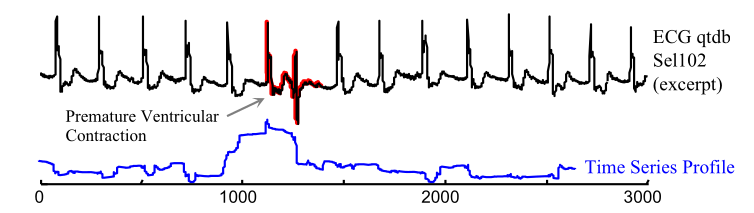
\includegraphics[width=0.8\linewidth]{Figures/MP_anomaly_detection.png}
    \caption{Ανχίχνευση ανωμαλιών με τον \emph{Matrix Profile} (αναπαραγωγή από \cite{yeh2018time})}
    \label{figure:MP}
\end{figure}

Για τον υπολογισμό του \emph{Distance Profile}, ο \emph{MP} χρησιμοποιεί τον αλγόριθμο \emph{MASS}, ο οποίος βασίζεται στον \emph{Fast Fourier Transform} (FFT). Με αυτόν τον τρόπο, η χρονική πολυπλοκότητα του υπολογισμού του \emph{Distance Profile} είναι $O(nlog n)$.
Έπειτα, για τον υπολογισμό ολόκληρου του \emph{Matrix Profile}, υπάρχουν 3 διαφορετικές μεθόδοι που ανέπτυξαν οι ερευνητές του \emph{MP}:
\begin{itemize}
    \item \emph{\strong{STAMP} (Scalable Time series Anytime Matrix Profile)}: Αυτός ο αλγόριθμος, υπολογίζει το \emph{Distance Profile} για κάθε υπακολουθία με τυχαία σειρά. Έτσι, ο χρήστης μπορεί ανά πάσα στιμγή να διακόψει την εκτέλεση του αλγορίθμου, και να πάρει μία προσέγγιση του \emph{Matrix Profile}. Η χρονική πολυπλοκότητα ανέρχεται σε $O(n^2log n)$, αλλά με βάση τα πειράματα των δημιουργών, η τελική χρονική πολυπλοκότητα είναι $O(n^2)$. Μία πιθανή εξήγηση για το παραπάνω συμβάν, είναι πως επειδή ο \emph{FFT} είναι πολύ σημαντικός σε πάρα πολλές εφαρμογές, είναι υπερβολικά πολύ βελτιστοποιημένος.
\item  \emph{\strong{STOMP} (Scalable Time series Ordered-search Matrix Profile)}: Είναι μία πιο γρήγορη παραλλαγή του \emph{STAMP} αν ο χρήστης διατίθεται να θυσιάσει το χαρακτηριστικό του \emph{anytime}. Η παραλλαγή αυτή, σαρώνει την χρονοσειρά με αυστηρή σειρά, από την αρχή προς το τέλος. Αυτό είναι σημαντικό, καθώς οι δημιουργοί του \emph{MP} παρατήρησαν πως για να βρεις το εσωτερικό γινόμενο $QT_{j,i}$ όπου $Q:$ η προς εξέταση υπακολουθία, μεταξύ 2 μετατοπισμένων υπακολουθιών κατά μία θέση, αρκεί να υπολογίσεις το προηγούμενο εσωτερικό γινόμενο $QT_{j-1,i-1}$ αφαιρόντας το παλαιότερο σημείο και προσθέτοντας το νεότερο, σε μόλις $O(1)$. Έτσι, η τελική χρονική πολυπλοκότητα του \emph{STOMP} είναι $O(n^2)$.
\item \emph{\strong{STOMPI} (Stomp Incremental)}: Παραλλαγή του \emph{STOMP}, η οποία δουλεύει για ροές δεδεομένων. Δεν επαναυπολογίζει ολόκληρο τον \emph{MP} από την αρχή, παρά μόνο ενημερώνει τα αποτελέσματα με βάση τα καινούργια δεδομένα. Η χρονική πολυπλοκότητα του \emph{STOMPI} είναι $O(n)$, όπου $n$ είναι το μήκους της μέχρι τώρα ακολουθίας. Αυτό συνεπάγεται, πως για κάθε σημείο που προστίθεται, ο αλγόριθμος γίνεται όλο και πιο αργός. Άρα ο καλύτερος τρόπος για να εξετάσουμε την απόδοσή του, είναι να μελετήσουμε τον \strong{Μέγιστο Χρονικό Ορίζοντα (ΜΗΤ)}. Θεωρόντας ένα παράδειγμα, όπου ένα dataset ενημερώνεται κάθε 8 δευτερόλεπτα, ο \emph{STOMPI} θα μπορούσε να τρέξει για 25 χρόνια. Αυτή η εκτίμηση που δίνουν οι ερευνητές είναι, χωρίς να συμπεριλάβουμε τις βελτιστοποιήσης που συμβαίνουν συνεχώς στο hardware.
\end{itemize}

Αν και στις περισσότερες περιπτώσεις, οι παραπάνω αλγόριθμοι θα μας κάλυπταν, υπάρχουν και κάποιοι κλάδοι, όπως αυτός των σεσμολόγων, οι οποίοι θα ήθελαν να έχουν απεριόριστο όριο στα δεδομένα τους. Για τέτοιους σκοπούς συγκεκριμένα, οι ερευνητές μετέφεραν τον \emph{STAMP} σε \emph{CUDA C++}, εκμεταλλευόμενοι της τεράστιες δυνατότητες για παράλληλισμό των επεξεργαστών της \emph{NVDIA}.

Ένα από τα πλεονεκτήματα που αναφέραμε προηγουμένος, είναι πως μπορούμε να γνωρίζουμε εκ των προτέρων, πόσο χρόνο θα χρειαστεί για να εκτελέσουμε τον \emph{MP}. Αυτό το επιτυγχάνουμε κάνοντας αρχικά ένα δοκιμαστικό έλεγχο στο μηχάνημά μας, υπολογίζοντας πόσο χρόνο $\delta$ θα κάνει για να υπολογίσει το \emph{MP} σε μία τυχαία χρονοσειρά μεγέθους $n$. Έπειτα για μία καινούργια χρονοσειρά μεγέθους $n_{new}$
το καινούργιο $\delta_{new}$ υπολογίζεται ως εξής:
$$\delta_{new} = \frac{\delta}{n^2} \times n_{new}^2$$

\begin{figure}
    \centering
    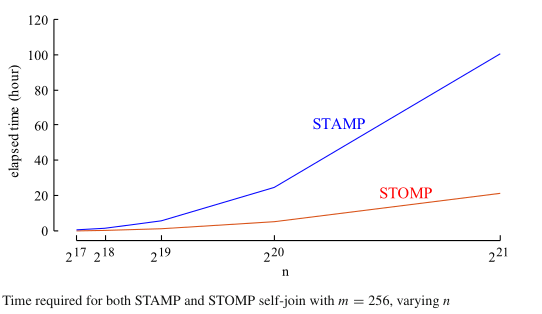
\includegraphics[width=0.8\linewidth]{Figures/stamp_stomp_varryingN.png}
    \caption{(αναπαραγωγή από \cite{yeh2018time})}
    \label{figure:STAMP-STOMP-VarN}
\end{figure}

Σημαντικό είναι να δούμε, τους απαιτούμενους χρόνους για τον \emph{STAMP} και τον \emph{STOMP}, όταν κρατάμε σταθερή την μία από τις 2 παραμέτρους ($n,m$).Παρατηρούμε στο σχήμα \ref{figure:STAMP-STOMP-VarN} πως ο \emph{STOMP} έχει σημαντικά καλύτερους χρόνους εκτέλεσης από τον \emph{STAMP} όσο μεγαλώνει το μέγεθος της χρονοσειράς. Το πιο σημαντικό όμως είναι, όπως φαίνεται στο σχήμα \ref{figure:STAMP-STOMP-VarM}, πως και οι 2 αλγόριθμοι, είναι σχεδόν σταθεροί ανεξαρτήτως του μεγέθους $m$ της υπακολουθίας. Μάλιστα φαίνεται να υπάρχει μία ελαφρώς φθίνουσα πορεία, όσο μεγαλώνει το $m$. Αυτό συμβαίνει διότι όσο μεγαλώνει το $m$, ο αριθμός των συγκρίσεων γίνεται όλο και μικρότερος.  

\begin{figure}
    \centering
    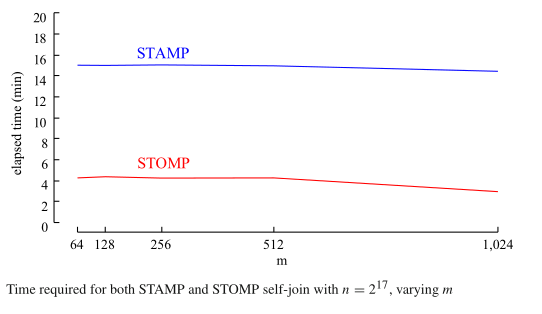
\includegraphics[width=0.8\linewidth]{Figures/stamp_stomp_varryingM.png}
    \caption{(αναπαραγωγή από \cite{yeh2018time})}
    \label{figure:STAMP-STOMP-VarM}
\end{figure}

Γενικά ο \emph{MP}, είναι μία από τις ταχύτερες/ακριβέστερες μεθόδους ανίχνευσης μοτίβων/ανωμαλιών, η οποία παρουσιάζει όμως ένα αδύνατο σημείο, το οποίο τονίζουν και οι ερευνητές του. Όταν υπάρχουν επαναλαμβανόμενες ανωμαλίες μέσα στα δεδομένα, μπορεί να θεωρήσει αυτά τα μοτίβα ως φυσιολογικά, διότι βασίζεται αυστηρά στην απόσταση του 1ου κοντινότερου γείτονα. Για παράδειγμα, αν σε εά ηλεκτροκαρδιογράφημα, ένας ασθενής έχει επαναλαμβανόμενες αρυθμίες, αυτές θα σημανθούν ως κανονικές, κάτι το οποίο δεν είναι επιθυμητό. Το παραπάνω γεγονός επιβεβαιώθηκε και από τους δημιουργούς του \emph{TSB-UAD}.

\subsection{POLY}
Ο αλγόριθμος \emph{POLY} \cite{li2007unifying} για την εύρεση ανωμαλιών σε χρονοσειρές, σε αντίθεση με άλλους αλγορίθμους οι οποίοι απαιτούν να είναι γνωστό εκ των προτέρων του τύπου του μοντέλου της χρονοσειράς ή είναι αρκετά ευαίσθητοι σε υπερπαράμετρους, αντιμετωπίζει το πρόβλημα με διαφορετική προσέγγιση. Χρησιμοποιόντας την τεχνική της Τοπικής Πολυωνυμικής Προσαρμογής (Local Polynomial Fitting), αποφεύγοντας την ανάγκη για παραμέτρους, και με την βοήθεια του \emph{Ασαφή Διαχωρισμού} και της \emph{Θεωρίας Λήψης Αποφάσεων}, μπορεί να εντοπίσει ανωμαλίες σε online χρονοσειρές, αλλά και σημεία αλλάγης (change points).

Οι ανωμαλίες και τα σημεία αλλαγής, μπορούν να περιγραφούν μέσω της συνολικής κανονικότητας του συστήματος (holistic regularity). Έτσι, οι δημιουργοί του \emph{POLY} ορίζουν σαν ανωμαλία, ένα σημείο το οποίο αποκλίνει σημαντικά από την συνολική κανονικότητα της χρονοσειράς, ενώ εά σημείο αλλαγής, αποτελεί το χρονικό σημείο από το οποίο και μετά, αλλάζει ολόκληρη η συνολική κανονικότητα της χρονοσειράς.

Για να ποσοτικοποιήσουν μαθηματικά αυτήν την συμπεριφορά, εξετάζουν δύο δύο δεσμευμένες πυκνότητες πιθανότητας για κάθε σημείο $x_t$ της χρονοσειράς:
\begin{itemize}
    \item \strong{Forward Conditional Density}: η οποία υπολογίζεται βάσει ενός παραθύρου δεδομένων του παρελθόντος $p(x_t|x_{t-L},...,x_{t-1})$.
    \item \strong{Backward Conditional Density}: η οποία υπολογίζεται βάσει ενός παραθύρου δεδομένων του μέλλοντος $p(x_t|x_{t+1},...,x_{t+L})$.
\end{itemize}

Οι παραδοσιακές μεθόδοι, προσπαθούσαν να υπολογίσουν αυτές τις πυκνότητες, προσαρμόζοντας τα δεδομένα τους σε αυστηρά καθολικά παραμετρικά μοντέλα. Κάτι τέτοιο όμως δεν είναι δυνατόν για χρονοσεριές, και έτσι οι δημιουργοί του \emph{POLY} υιοθέτησαν την τεχνική της Τοπικής Πολυωνυμικής Προσαρμογής, όπου για κάθε χρονικό σημείο, απομονώνεται μόνο ένα μικρό τοπικό παράθυρο, όπου ο αλγόριθμος προσπαθεί να ταιριάξει μία απλή τοπική καμπύλη. Βάση αυτής της καμπύλης ο αλγόριθμος υπολογίζει ποιά θα έπρεπε να είναι αναμενόμενη τιμή του σημείου που εξετάζεται.

Έχοντας πλέον την δυνατότητα να προβλέψει την αναμενόμενη τιμή κάθε σημείου μέσω των τοπικών πολυωνύμων, ο αλγόριθμος πρέπει να αποφασίσει αν ενα σημείο είναι ανώμαλο/σημείο αλλαγής ή όχι. Αρχικά, για κάθε σημείο υπολογίζει δύο βαθμολογίες, την \emph{Forward Score} και την \emph{Backward Score}, όπου είναι ίσες με το τετράγωνο της διαφοράς μεταξύ της πραγματικής και της εκτιμώμενης τιμής του σημείου, διαιρούμενη με την διακύμανση των δεδομένων του παραθύρου.

Ωστόσο, η απόφαση για το αν ένα σημείο είναι ανώμαλο/σημείο αλλαγής, δεν γίνεται απλά με βάση κάποιο κατώφλι, αλλά υιοθετείται μία διαφορετική λογική, η οποία πηγάζει από τα \emph{Ασαφή Σύνολα}. Το σύστημα χρησιμοποιώντας τις αρχικές βαθμολογίες, και δύο σταθερές ανοχής, δεν απορρίπτει ούτε αποδέχεται απόλυτα εά σημείο, αλλά υπολογίζει τον βαθμό συμμετοχής του, σε τέσσερις διαφορετικές καταστάσεις, όπως φαίνονται παρακάτω:
\begin{itemize}
    \item \strong{FNormalX}: Το σημείο θεωρείται φυσιολογικό σε σχέση με τα δεδομένα του παρελθόντος.
    \item \strong{BNormalX}: Το σημείο θεωρείται φυσιολογικό σε σχέση με τα δεδομένα του μέλλοντος.
    \item \strong{NotFNormalX}: Το σημείο δεν θεωρείται κανονικό σε σχέση με τα δεδομένα του παρελθόντος.
    \item \strong{NotBNormalX}: Το σημείο δεν θεωρείται κανονικό σε σχέση με τα δεδομένα του μέλλοντος.
\end{itemize}

Έπειτα δημιουργούνται 2 ασαφή σύνολα:
\begin{itemize}
    \item \strong{Outlier Set}: όπου $Outlier = NotFNormalX \cap NotBNormalX$ και ανήκουν τα ανώμαλα σημεία της χρονοσειράς.
    \item \strong{Change Point Set}: όπου $Change = NotFNormalX \cap BNormalX$ και ανήκουν τα σημεία αλλαγής της χρονοσειράς.
\end{itemize}

Οι κύριες ρυθμίσεις που απαιτούνται για τον \emph{POLY} είναι το μέγεθος του παραθύρου $h$ και ο βαθμός του τοπικού πολυωνύμου $p$. Οι δημιουργού του, προτείνουν ο βαθμός του πολυωνύμου να είναι περιττός αριθμός (π.χ. $p=1$, $p=3$), καθώς από πειράματα που έκαναν, παρατήρησαν ότι προσφέρει καλύτερη προσαρμογή στα δεδομένα.Το μέγεθος του παραθύρου $h$ μπορεί να υπολογιστεί δυναμικά, όπου σαν αρχικές τιμές δίνουν $h=[X^f_{max} - X^f_{min}]/(L-1)$ για την εμπρόσθια εκτίμηση, και $h=[X^b_{max} - X^b_{min}]/(L-1)$ για την οπίσθια εκτίμηση, αναπροσαρμόζοντάς τας με έναν παράγοντα $C=1.1$, μέχρι το $MISE(h)\leq\delta$, όπου $\delta$ είναι ένα κατώφλι για το $MISE$.

 
% Chapter 3

\chapter{Πειραματική Διάταξη και Συγκριτική αξιολόγηση} % Main chapter title

\label{Chapter3} % For referencing the chapter elsewhere, use \ref{Chapter3} 
%----------------------------------------------------------------------------------------

% Define some commands to keep the formatting separated from the content 


%----------------------------------------------------------------------------------------

\section{Γενικά}

Σκοπός αυτού του κεφαλαίου είναι να πραγματοποιηθεί μία συστηματική αξιολόγηση των αλγορίθμων που παρουσιάστηκαν στο προηγούμενο κεφάλαιο, σε σχέση με το σύστημα \emph{Auto-TSAD}, κάτω από ένα τυποποιημένο πρότυπο αναφοράς, όπως το \emph{TSB-UAD}.

Τα δεδομένα τα οποία χρησιμοποιήθηκαν για την εκτέλεση των πειραμάτων ήταν από 2 datasets τα οποία είχαν συλλεχτεί από τους δημιουργούς του \emph{TSB-UAD}, το \emph{public\_v2} το οποίο υπάρχει διαθέσιμο στο \href{https://www.thedatum.org/datasets/TSB-UAD-Public-v2.zip}{public\_v2 dataset} καθώς και το \emph{Artificial dataset} το οποίο είναι διαθέσιμο στο \href{https://www.thedatum.org/datasets/TSB-UAD-Artificial.zip}{artificial dataset}. 

Για κάθε dataset έγιναν 2 διαφορετικά πειράματα στο \emph{Auto\_TSAD}, ένα με ενεργοποιημένη την μηχανή βελτιστοποίησης \emph{optuna}, η οποία απαιτούσε αρκετό χρόνο για να εκτελέσει ένα πείραμα, και ένα με κλειστή την μηχανή βελτιστοποίησης. Έτσι o αριθμός των χρονοσειρών που εκτελέστηκαν σε κάθε πείραμα, έχουν όπως στον πίνακα \ref{tab:experiments_num}:

\begin{table}[h]
\centering
\caption{Experiments For Auto-TSAD with/out for each dataset}
\label{tab:experiments_num}
\begin{tabular}{lcc}
\toprule
Dataset & Optuna-ON & Optuna-OFF \\
\midrule
Public V2 & 29 & 3429 \\
Artificial & 236 & 960 \\
\bottomrule
\end{tabular}
\end{table}
\subsection{Μετρικές Αξιολόγησης}
Οι μετρικές που αξιολογήθηκαν ήταν ο χρόνος που απαιτήθηκε, καθώς και το score που πέτυχε η κάθε τεχνική με βάση την μετρική \strong{VUS-ROC}. O χρόνος σε συνάρτηση με την \emph{ROC-VUS} είναι σημαντικά, καθώς μας επιτρέπει να αξιολογήσουμε αν η διαφορά στον εντοπισμό των ανωμαλιών είναι αρκετά μεγάλη, για να δικαιολογήσει και το χρονικό κόστος που απαιτεί η μηχανή βελτιστοποίησης \emph{optuna} του \emph{Auto-TSAD}.

\subsection{Γενικές Παρατηρήσεις}
Σαν μία γενική πρώτη παρατήρηση είναι πως το \emph{Auto-TSAD} δεν μπορεί να αποδόσει σωστά χωρίς να έχουμε ενεργοποιήσει την \emph{optuna}. Συγκεκριμένα, το ποσοστό επιτυχίας του, ώστε να μπορέσει να βρει έστω και μία ανωμαλία, ήταν πολυ χαμηλό όταν δεν ήταν ενεργοποιημένη η \emph{optuna}. Τα αποτελέσματα φαίνονται στο Σχήμα \ref{figure:success_rates_tsad}. Παρατηρούμε τόσο στο \emph{Public} όσο και στο \emph{Artificial} dataset, το ποσοστό επιτυχίας ανίχνευσης έστω και μίας ανωμαλίας αγγίζει το $100\%$ όταν η \emph{optuna} είναι ενεργοποιημένη, ενώ αντιθέτως τα ποσοστά επιτυχίας είναι πολύ πιο χαμηλά με τιμές $31,2\%$ για το \emph{Public} και $9,2\%$ για το \emph{Artificial} dataset.
Συγκεκριμένα, χωρίς την \emph{optuna} ενεργοποιημένη, το σύστημα \emph{Auto-TSAD} δεν μπόρεσε να πάραξει κανένα αποτέλεσμα, για καμία μετρική. Το σύστημα \emph{Auto-TSAD} υπολογίζει την απόδοση στις παρακάτω μετρικές:

\begin{itemize}
    \item PrAUC
    \item RocAUC
    \item RangePrAUC
    \item RangeRocAUC
    \item RangePrVUS
    \item RangeRocVUS
    \item RangePrecision
    \item RangeRecall
    \item RangeFScore
    \item Precision
    \item Recall
    \item FScore
    \item PrecisionAtK
\end{itemize}

\begin{figure}[h]
    \centering
    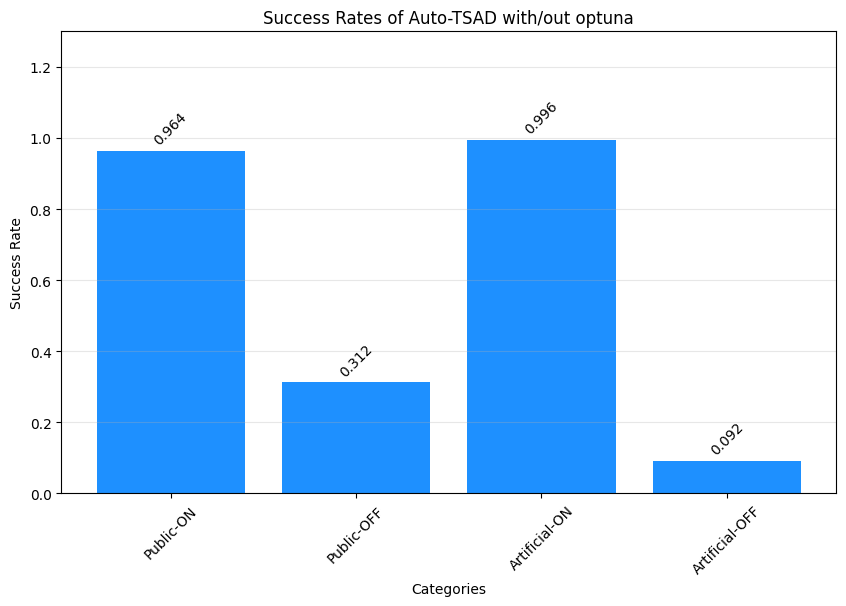
\includegraphics[width=1\linewidth]{Figures/success_rates_tsad.png}
    \caption{Ποσοστά επιτυχίας ανίχνευσης τουλάχιστον μίας ανωμαλίας του Auto-TSAD}
    \label{figure:success_rates_tsad}
\end{figure}

\subsection{TODO}
\textcolor{red}{TODO ΓΙΑΤΙ ΔΕΝ ΕΠΙΣΤΡΕΦΕΙ ΟΜΩΣ ΑΠΟΤΕΛΕΣΜΑΤΑ? ΔΕΝ ΕΙΝΑΙ ΠΕΡΙΟΔΙΚΑ??}
 
\section{Public Dataset}
Σε αυτό το κεφάλαιο θα συγκρίνουμε τα αποτελέσματα του \emph{Auto-TSAD} με τις άλλες μετρικές \emph{IForesit - POLY - MP}.
Για το \emph{Auto-TSAD}, με ανοιχτή την μηχανή βελτιστοποίησης \emph{optuna}, επιλέχτηκε τυχαία μία χρονοσειρά από κάθε dataset, ενώ με κλειστή την μηχανή \emph{optuna}, ο \emph{Auto-TSAD} έτρεξε στο σύνολο των χρονοσειρών. Οι μετρικές \emph{IForest - POLY - MP} εκτελέστηκαν μόνο στις ίδιες επιλεγμένες χρονοσειρές που έτρεξε και ο \emph{Auto-TSAD}.

\subsection{Τα dataset}
Τα dataset που επιλέχτηκαν από τους δημιουργούς του \emph{Auto-TSAD}, καλύπτουν μία ευρεία γκάμα από διαφορετικούς τομείς, με διαφορετικούς τύπους ανωμαλιών. Πιο συγκεκριμένα:
\begin{itemize}
    \item \emph{Genesis}: Προέρχεται από έναν φορητό επιδείτη τοποθέτησης και μεταφοράς, ο οποίος χρησιμοποιεί μία δεξανμενή αέρα για να τροφοδοήσει ρομποτικές μονάδες λαβής και αποθήκευσης. Περιέχει ακολουθίες ανωμαλιών.
    \item \emph{WSD}: Αφορά χρονοσειρές που συλλέγουν δεδομένα από μεγάλες εταιρίες του Διαδικτύου, και περιέχουν Βασικούς Δείκτες Απόδοσης. Περιέχει ακολουθίες ανωμαλιών.
    \item \emph{MSL}: Συλλογή δεδομένων της NASA που προέρχονται από τους αισθητήρες του Rover Curiosity από τον Άρη. Περιέχει ακολουθίες ανωμαλιών.
    \item \emph{Stock}: Αφορά δεδομένα από αγορές μετοχών.Περιέχει ανωμαλές σημείων.
    \item \emph{Dapnhet}: Ιατρικά δεδομένα που σχετίζονται με την νόσο του Parkinson. Καταγράφει ενδείξεις από 3 αισθητήρες επιτάχυνσης οι οποίοι είναι τοποθετημένοι στο ισχύο και στο πόδι ασθενών, και εντοπίζουν το φαινόμενο freezing of gate (FoG) κατά τη διάρκεια εργασιών περπατήματος. Περιέχει ακολουθίες ανωμαλιών.
    \item \emph{MITDB}: Αφορά δεδομένα που συλλέχτηκαν από 47 ασθενής, και περιέχει 48 αποσπάσματα μισής ώρας ηλεκτροκαρδιογραφημάτων διπλού καναλιού, και προσπαθούν να εντοπίσουν καρδιακές αρυθμίες. Περιέχει ακολουθίες ανωμαλιών.
    \item \emph{GHL}: Αφορά δεδομένα τα οποία συλλέγονται από 3 δεξαμενές σε έναν βρόγχο θέρμανσης πετρελαίου. Καταγράφει την θερμοκρασία και την στάθμη τους. Οι ανωμαλίες αντιστοιχούν σε αλλαγές στην μέγιστη θερμοκρασία ή την συχνότητα της αντλίας. Πρόκειται για ακολουθίες ανωμαλιών.
    \item \emph{Sensorscope}: Μία συλλογή από περιβαλλοντικά δεδομένα που αφορούν θερμοκρασία, υγρασία, ηλιακή ακτινοβολία κ.ο.κ. Πρόκειται για ακολουθίες ανωμαλιών.
    \item \emph{SMD}: Δεδομένα καταγραφής λειτουργίας 28 διαφορετικών server, 3 διαφορετικών ομάδων, διάρκειας 5 εβδομάδων από μεγάλη εταιρία Διαδικτύου. Περιέχει ακολουθίες ανωμαλιών.
    \item \emph{MGAB}: Αποτελείται από χρονοσειρές Mackey-Grass, η οποίες παρουσιάζουν χαοτική συμπεριφορά, κάνοντας πολύ δύσκολο το έργο ανίχνευσης ανωμαλιών με γυμνό μάτι. Περιέχει ακολουθίες ανωμαλιών.
    \item \emph{NAB}: Σύνθετα δεδομένα από πραγματικές και τενητές χρονοσειρές, οι οποίες προέρχονται από διάφορους server, όπως AWS, αναφορές στο \emph{X} σε μεγάλες εισηγμένες εταιρίες κ.ο.κ. Περιλαμβάνει ακολουθίες ανωμαλιών.
    \item \emph{SED}: Αφορά δεδομένα από δίσκους κινητήρων της NASA σε διάφορες φάσης λειτουργίας, σε σταθέ ταχύτητα $3000 rpm$. Αφορά ακολουθίες ανωμαλιών.
    \item \emph{SVDBM}: Περιλαμβάνει 78 ιατρικά καρδιογραφήματα, ημίωρης διάρκειας, επιλεγμένες ειδικά για να συμπληρώσουν το \emph{MITB}. Περιέχει ακολουθίες ανωμαλιών.
    \item \emph{Dodgers}: Δεδομένα καταγραφής κίνησης στον αυτοκινητόδρομο 101 του LA, μετά το τέλος αγώνα της ομάδας μπέιζμπολ Dodgers. Περιέχει ακολουθίες ανωμαλιών.
    \item \emph{TAO}: Δεδομένα που αφορούν μετεωρολογικές και ωκεανογραφικές μετρήσεις. Περιέχει και μεμονωμένες ανωμαλίες αλλά και ακολουθίες ανωμαλιών.
    \item \emph{IOPS}: Δεδομένα που αφορούν την ποιότητα των διαδικτυακών υπηρεσιών και την υγεία ενός μηχανήματος. Περιέχει ακολουθίες ανωμαλιών.
    \item \emph{OPPORTUNITY}: Αφορά αισθητήρες οι οποίοι συλλέγουν δεδομένα κατά την ανθρώπινη δραστηριότητα. Περιέχει ακολουθίες ανωμαλιών.
    \item \emph{NEK}: Περίεει δεδομένα από διαδικτυακές συσκευές παραγωγής. Περιέχει τόσο σημειακές ανωμαλίες όσο και ακολυθίες ανωμαλιών.
    \item \emph{CreditCard}: Αφορά δεδομένα συναλλαγών μέσω πιστωτικών καρτών. Προσπαθεί να εντοπίσει απάτες. Περιέχει μεμονωμένες ανωμαλίες καθώς και ακολουθίες ανωμαλιών.
    \item \emph{CATSv2}: Περιλαμβάνει δεδομένα από εντολές συστήματος, εξωτερικά ερεθίσματα και μετρήσεις τηλεμετρίας, στις οποίες έχουν εισαχθεί 200 ανωμαλίες. Περιέχει ακολουθίες ανωμαλιών.
    \item \emph{TODS}: Συνθετικό dataset το οποίο περιέχει διαφορετικού τύπου δεδομένων για την αξιολόγηση αλγορίθμων εύρεσης ανωμαλιών. Περιέχει τόσο μεμονωμένες ανωμαλίες καθώς και ακολουθίες ανωμαλιών.
    \item \emph{Power}: Καταγράφει δεδομένα ζήτησης/κατανάλωσης ενέργειας. Περιέχει ακολουθίες ανωμαλιών.
    \item \emph{UCR}: Συλλογή από διάφορες μονοσδιάστατες χρονοσειρές, από διάφορους τομείς, στις οποίες οι περισσότερες ανωμαλίες έχουν εισηχθή τεχνητά. Περιέχει και μεμονωμένες ανωμαλίες αλλά και ακολυθίες ανωμαλιών.
    \item \emph{SMAP}: Πραγματικά δεδομένα από καταγραφές και μετρήσεις αεροδιαστημικών συστημάτων και δορυφόρων. Περιέχει ακολουθίες ανωμαλιών.
    \item \emph{SWaT}: Περιλαμβάνει δεδομένα τα οποία προέρχονται από 51 ασθητήρες και ενεργοποιητές, όπου αναλύουν το νερό. Οι ανωμαλίες αντιπροσωπεύουν λάθος ενδείξεις στις μετρήσεις των αισθητήρων λόγο κυβερνοεπιθέσεων. Περιέχει ακολουθίες ανωμαλιών.
    \item \emph{YAHOO}: Περιλαμβάνει δεδομένα τα οποία προέρχονται από τα εργαστήρια της YAHOO και αφορά πραγματικές και συνθετικές χρονοσειρές, βασισμένες στην πραγματική κίνηση παραγωγής διάφορων συστημάτων της εταιρίας. Περιέχει τόσο μεμονωμένες ανωμαλίες, αλλά και ακολουθίες ανωμαλιών.
    \item \emph{GECCO}: Dataset το οποίο αφορά στην ποιότητα του νερού, για online ανίχνευση ανωμαλιών. Περιέχει ακολουθίες ανωμαλιών.
    \item \emph{EXATHLON}: Δεδομένα από πραγματικα ίχνη δεδομένων, τα οποία συλλέχτηκαν επί 2,5 μήνες από ένα Spark cluster. Για κάθε ανωμαλία παρέχονται ακριβές ετικέτες τόσο για το χρονικό διάστημα της βασικής αιτίας, αλλά και για το χρονικό διάστημα των επιπτώσεων. Περιέχει ακολουθίες ανωμαλιών.
\end{itemize}
\subsection{Χρόνοι εκτέλεσης}
Τα πειράματα εκτελέστηκαν σε τρία μηχανήματα με λειτουργικό σύστημα Fedora Linux 43. Το πρώτο μηχάνημα διέθετε επεξεργαστή Intel Core i5-10400 (6 πυρήνες, 4GHz), κάρτα γραφικών AMD Radeon RX 5700 XT και 16GB μνήμης RAM DDR4. Τα υπόλοιπα δύο μηχανήματα ήταν ίδια μεταξύ τους, με επεξεργαστή Intel Core i5-9500T (6 πυρήνες, 2.2GHz), ενσωματωμένη κάρτα γραφικών Intel UHD Graphics 630 και 16GB μνήμης RAM DDR4.

Όπως αναφέρθηκε και προηγουμένως, σημαντικό είναι να εξετάσουμε τους χρόνους εκτέλεσης. Η μηχανής βελτιστοποίησης της \emph{optuna}, που χρησιμοποιεί το \emph{Auto-TSAD} απαιτεί αρκετό χρόνο για να υπολογίσει και να βρει τις καλύτερες υπερπαράμετρους για τον κάθε αλγόριθμο, ώστε να καταλήξει στην χρήση ενός αλγόριθμου με τις καλύτερες δυνατές υπερπαραμέτρους. Τα αποτελέσματα φαίνονται συγκεντρωτικά στο Σχήμα \ref{figure:time_optuna_on}. Ο μέγιστος χρόνος εκτέλεσης που παρατηρήθηκε, ήταν 37,1 ώρες (37 ώρες και 6 λεπτά) για το dataset \emph{TAO}, ενώ ο ελάχιστος χρόνος ήταν 0,4 ώρες (24 λετπά). Επίσης η μέση τιμή είναι 3,84 ώρες (3 ώρες και 50 λεπτά) και η τυπική απόκλιση είναι 7,35 ώρες (7 ώρες και 21 λεπτά). Συγκεντρωτικά όλα τα στατιστικά στοιχεία φαίνονται στον πίνακα.

\begin{figure}[h]
    \centering
    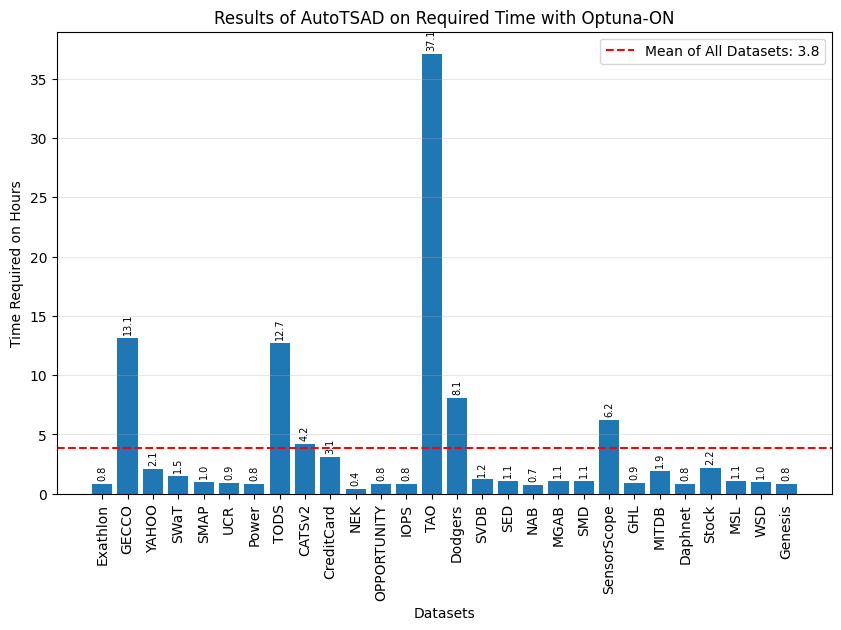
\includegraphics[width=1\linewidth]{Figures/v2_time_optuna-on_tsad.png}
    \caption{Χρόνοι εκτέλεσης για κάθε dataset με ανοιχτή την μηχανή βελτιστοποίησης optuna, σε ώρες.}
    \label{figure:time_optuna_on}
\end{figure}

\begin{table}[h]
\centering
\caption{Στατιστικά χρόνου εκτέλεσης με την optuna στο publicv2 dataset}
\label{tab:statistics-optuna-on}
\begin{tabular}{lc}
\toprule
Measure & Value \\
\midrule
Mean & 3.84  \\
std & 7.35 \\
min & 0.40 \\
25\% & 0.80 \\
50\% & 1.10 \\
75\% & 2.43 \\
max & 37.10\\ 
\bottomrule
\end{tabular}
\end{table}

Ενώ το 75\% των dataset εκτελούντε μέχρι 2 ώρες και 26 λεπτά, υπάρχουν και κάποια dataset όπως το \emph{GECCO, TODS, TAO, DODGERS και SensorScope} για τα οποία απαιτήθηκε πολύ παραπάνω χρόνος εκτέλεσης. Αυτά τα δεδομένα, δεν παρουσιάζουν όλα μαζί κάποιο ενιαίο χαρακτηριστικό, το οποίο να δικαιολογεί συνολικά τον τόσο αυξημένο χρόνο εκτέλεσής του. Παρ' όλα αυτά, μία πιθανή εξήγηση είναι η εξής:
\begin{itemize}
    \item To \emph{GECCO} και το \emph{DODGERS} έχουν σαν μέσο μήκος χρονοσειράς, 138.000 και 50.400 σημεία αντίστοιχα. Το \emph{Auto-TSAD} επειδή μπορεί να εκτελέσει τον κάθε αλγόριθμο μέχρι και 800 φορές για την εύρεση των καλύτερων υπερπαραμέτρων, σε συνδιασμό με τον μεγάλο όγκο των δεδομένων, μπορεί να εκτοξεύσει τους χρόνους εκτέλεσης.
    \item Το \emph{TAO} και το \emph{TODS}, ενώ δεν έχουν τόσο μεγάλο μήκος χρονοσειρών, φαίνεται ότι έχουν σχετικά υψηλό ποσοστό ανωμαλιών, με 9,4\% και 6,3\% αντιστοίχως, καθώς επίσης οι τύποι των ανωμαλιών που περιέχουν είναι και μεμονωμένες ανωμαλίες αλλά και ακολουθίες ανωμαλιών.
    \item Τέλος το \emph{SensorScope} αλλά και το \emph{DODGERS} παρουσιάζουν πολύ υψηλό ποσοστό ανωμαλιών με 22,5\% και 11,14\% αντίστοιχα.
\end{itemize}
Γενικά, φαίνεται πως αλγόριθμοι οι οποίοι δεν μπορούν να κλιμακώσουν σωστά σε μεγάλο σετ δεδομένων, ή με πολλές ανωμαλίες, δυσκολεύουν πάρα πολύ την μηχανή της Optuna και πολλές φορές αναγκάζεται να τρέξει σχεδόν όλες τις επαναλήψεις για όλους τους αλγορίθμους που χρησιμοποποιεί, καθώς δεν μπορεί να βρει 10 σετ υπερπαραμέτρων με απόδοση μεγαλύτερη του 95\% για να σταματήσει την λειτουργία της. 

Οι χρόνοι εκτέλεσης χωρίς ανοιχτή την μηχανή \emph{Optuna} είναι πολύ μικρότεροι, με μέσο χρόνο εκτέλεσης τα 3 λεπτά και τυπική απόκλιση 12 λεπτών. Ενδιαφέρον εύρημα αποτελεί ο μέγιστος χρόνος εκτέλεσης, ο οποίος ανέρχεται σε 6 ώρες και 41 λεπτά, o οποίος ανήκει στην χρονοσειρά με όνομα LTDB\textbackslash14157\_col\_0 η οποία βρέθηκε να έχει $9.5 \times 10^{6}$ σημεία. Τα αποτελέσματα βρίσκονται στον πίνακα \ref{optuna-off_runtime_pv2_with_outlier}. Αν επαναυπολογήσουμε τα καινούργια στατιστικά, χωρίς αυήν την ακράια τιμή, τότε η καινούργια μέση τιμή έιναι ίση με 167 sec, ενώ η καινούργια τυπική απόκλιση είναι 74 sec, όπως φαίνεται και στον πίνακα \ref{optuna-off_runtime_pv2_without_outlier}.
\begin{table}[h]
    \centering
    \caption{Χρόνοι εκτέλεσης σε sec στο dataset public v2, χωρίς ενεργή την μηχανή βελτιστοποίησης}
    \label{optuna-off_runtime_pv2_with_outlier} 
    \begin{tabular}{lc}
        \toprule
        Statistics & Runtimes in seconds \\
        \midrule
            mean & 190 \\
            std & 736 \\
            median & 54 \\
            min & 3 \\
            max & 24109 \\
        \bottomrule
    \end{tabular}
\end{table}

\begin{table}
    \centering
    \caption{Χρόνοι εκτέλεσης σε sec στο dataset public v2, χωρίς ενεργή την μηχανή βελτιστοποίησης και χωρίς ακραίες τιμές}
    \label{optuna-off_runtime_pv2_without_outlier} 
    \begin{tabular}{lc}
        \toprule
        Statistics & Runtimes in seconds \\
        \midrule
            mean & 167 \\
            std & 74 \\
        \bottomrule
    \end{tabular}
\end{table}

Όσον αφορά το \emph{TSB-UAD}, εξετάστηκαν οι χρόνοι εκτέλεσης των αλγορίθμων \emph{IForest - POLY} και \emph{MP}, καθώς δεν υπήρχε πρόσβαση στον αλγόριθμο \emph{NORMA} από τους δημιουργούς του \emph{TSB-UAD}. Η εφαρμογή τους έγινε πάνω στις ίδιες χρονοσειρές οι οποίες επιλέχτηκαν από το \emph{Auto-TSAD} με ενεργοποιημένη την μηχανή \emph{Optuna} για να βγουν όσο το δυνατό πιο αντικειμενικά αποτελέσματα. Ο υπολογισμός του χρόνου για κάθε αλγόριθμο, αφορά από την εκπαίδευση των μοντέλων μέχρι και την εξαγωγή των score, ενώ δεν συμπεριλήφθηκε ο υπολογισμός των μετρικών.Για την ανάπτυξη του κώδικα, χρησιμοποιήθηκε το notebook το οποίο υπάρχει στο github repository των δημιουργών του \emph{TSB-UAD}, το οποίο βρίσκεται στον σύνδεσμο \href{https://github.com/TheDatumOrg/TSB-UAD/blob/main/example/notebooks/test_anomaly_detectors.ipynb}{Anomaly detection for time series from TSB-UAD authors}. Ο κώδικας για την εκτέλεση των τριών αλγορίθμων έχει όπως στα Σχήματα \ref{figure:runIforest} έως \ref{figure:runMP}. TODO ΜΑΛΛΟΝ ΠΡΕΠΕΙ ΝΑ ΓΡΑΨΩ ΚΑΙ ΤΙ ΚΑΝΕΙ Ο ΚΩΔΙΚΑΣ ΕΔΩ !!!!!!!!!!!!!!!!!!!!!!   

\begin{figure}[h]
    \centering
    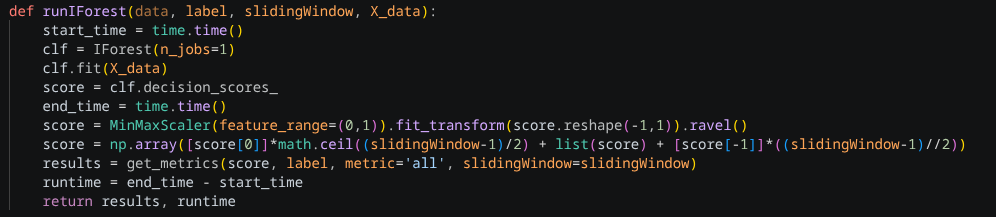
\includegraphics[width=1\linewidth]{Figures/run_IForest.png}
    \caption{Κώδικας για την εκτέλεση του IForest μέσω του TSB-UAD}
    \label{figure:runIforest}
\end{figure}

\begin{figure}[h]
    \centering
    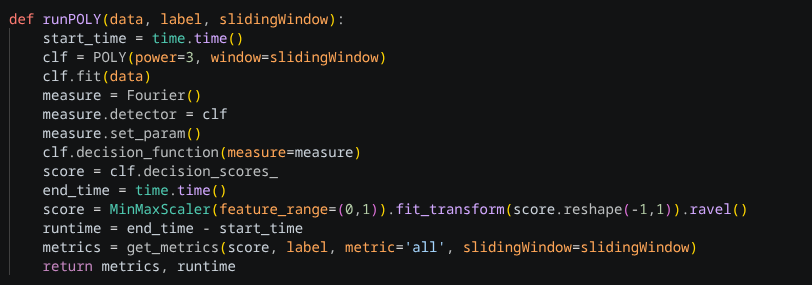
\includegraphics[width=1\linewidth]{Figures/runPOLY.png}
    \caption{Κώδικας για την εκτέλεση του POLY μέσω του TSB-UAD}
    \label{figure:runPOLY}
\end{figure}

\begin{figure}[h]
    \centering
    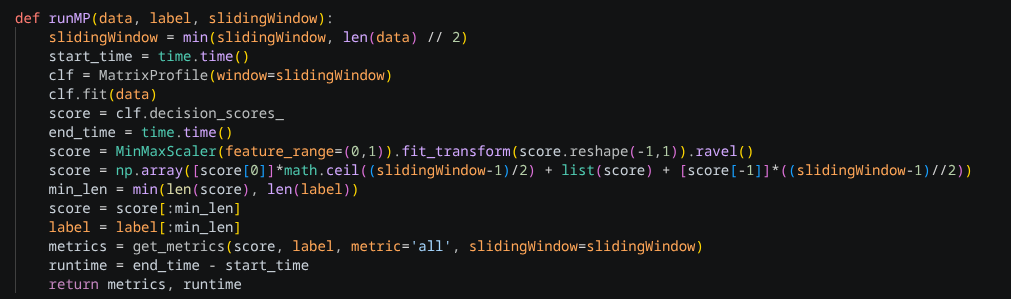
\includegraphics[width=1\linewidth]{Figures/runMP.png}
    \caption{Κώδικας για την εκτέλεση του MP μέσω του TSB-UAD}
    \label{figure:runMP}
\end{figure}

Οι απαιτήσεις εκτέλεσης αυτών των αλγορίθμων ήταν πολύ μικρές, της τάξης των 5-6 δευτερολέπτων μέγιστο για τους \emph{IForest} και \emph{POLY}, ενώ για τον \emph{MP} κάποιες φορές απαιτήθηκε παραπάνω χρόνος, με μέγιστες τιμές μέχρι και 800 δευτερόλεπτα. Σαν γενική εντύπωση είναι πως το \emph{TSB-UAD} χρειάστηκε αρκετά μικρότερο χρόνο (της τάξης των δευτερολέπτων μέχρι και κάποιων λεπτών) σε αντίθεση με το \emph{Auto-TSAD} το οποίο σε εξαιρετικές περιπτώσεις απαιτούσε ακόμα και μέρες για να παράξει αποτελέσματα. Στο σχήμα \ref{figure:tsb-times} παρουσιάζονται οι χρονικές απαιτήσεις του κάθε αλγορίθμου που εκτελέστηκαν μέσω του \emph{TSB-UAD}. Παρότι οι αλγόριθμοι που έτρεχαν στο \emph{TSB-UAD} απαιτούσαν σχεδόν μηδενικό χρόνο σε σύγκριση με \emph{Auto-TSAD}, είναι σημαντικό πως, όπως θα δούμε παρακάτω, όλοι κατάφεραν να παράξουν αποτελέσματα, δηλαδή να ανιχνέυσουν ανωμαλίες (το ποσοστό αποτυχίας ανίχνευσης ανωμαλιών του \emph{Auto-TSAD} με κλειστή την μηχανή της Optuna ήταν $\approx 69\%$).

\begin{figure}[h]
    \centering
    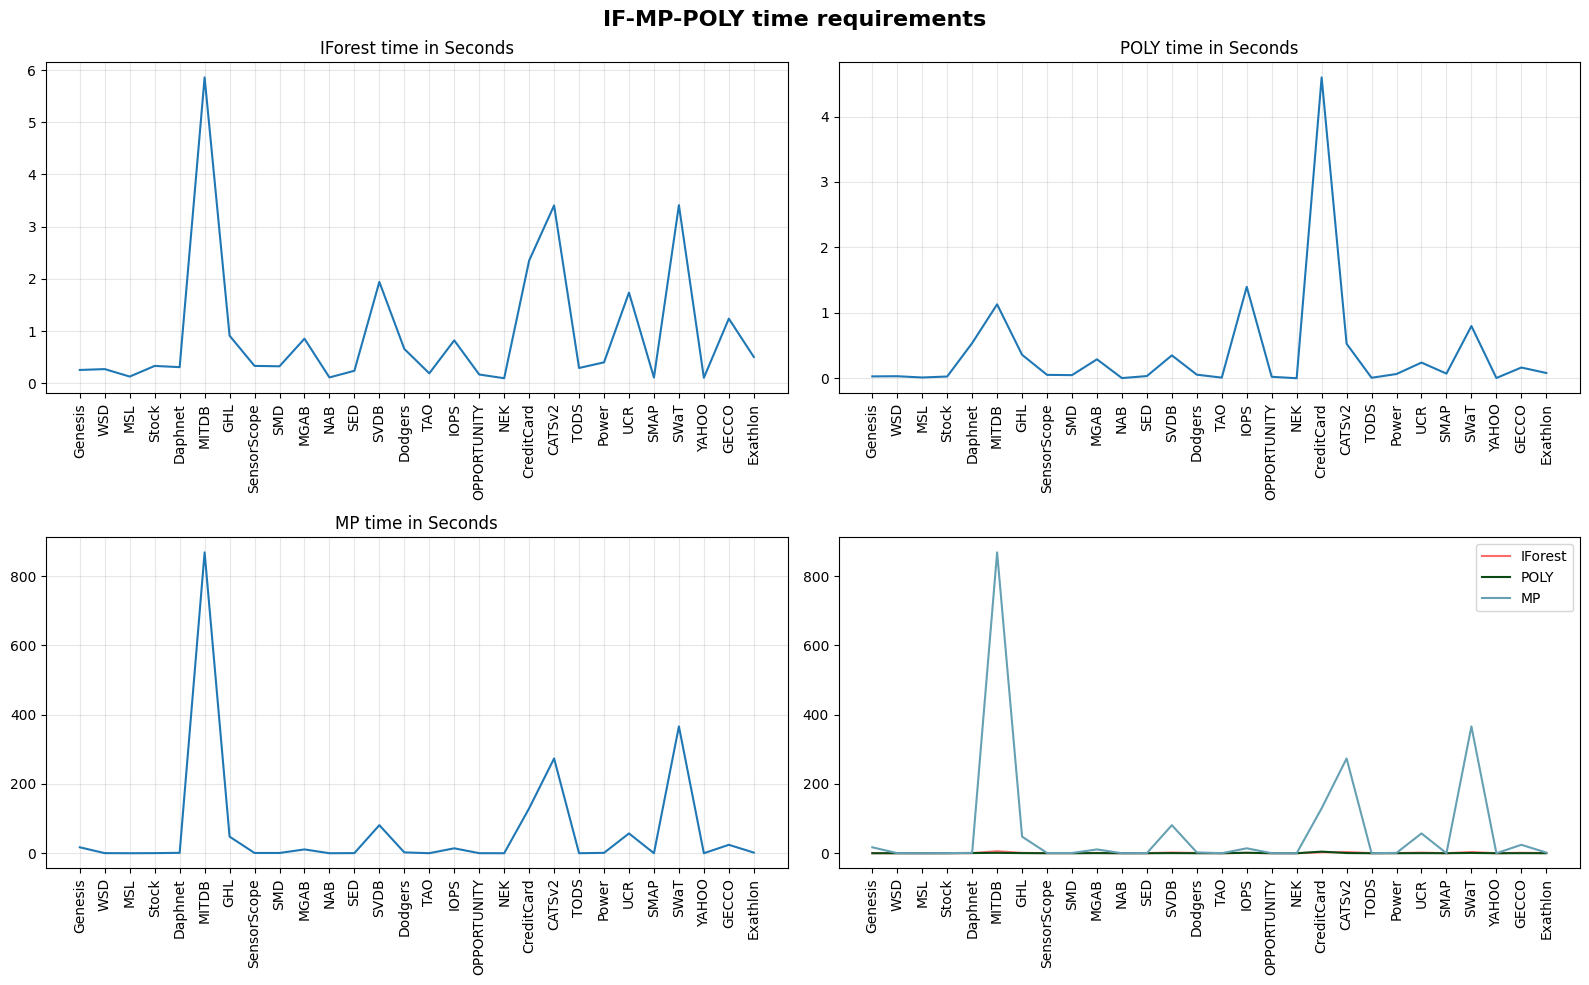
\includegraphics[width=1\linewidth]{Figures/v2_time_tsb.png}
    \caption{Κώδικας για την εκτέλεση του MP μέσω του TSB-UAD. 
        Πάνω αριστερά διακρίνουμε τις χρονικές απαιτήσεις του IForest. 
        Πάνω δεξιά της χρονικές απαιτήσεις του POLY. 
        Κάτω αριστερά διακρίνουμε τις χρονικές απαιτήσεις του MP. 
        Κάτω δεξιά διακρίνουμε συγκριτικά τις χρονικές απαιτήσεις όλων των αλγόριθμων.}
    \label{figure:tsb-times}
\end{figure}

\subsection{Αποτελέσματα ROC-VUS}
Θα εξετάσουμε τα αποτελέσματα της μετρικής \emph{ROC-VUS}:
\begin{enumerate}
    \item Mε ανοιχτή την Optuna και μεταξύ των αλγορίθμων που τρέχουμε στο \emph{TSB-UAD}
    \item Με κλειστή την Optuna και μεταξύ των αλγορίθμων που τρέχουμε στο \emph{TSB-UAD}
    \item Μεταξύ όλων των αποτελεσμάτων
\end{enumerate}
Έτσι θα έχουμε μία πιο σφαιρική άποψη για την επίδραση της Optuna στην εύρεση των ανωμαλιών.
\subsubsection{Συγκριτικά αποτελέσματα με Optuna-ON}

Τα αποτελέσματα της χρήσης της μηχανής της Optuna, είναι, όπως φαίνεται και στο Σχήμα \ref{figure:tsad-vus-on}, αρκετά εντυπωσιακά. Στα περισσότερα dataset, ανακάλυψε επιτυχημένα πάνω από το $90\%$ των ανωμαλιών, ενώ σημαντικό είναι επίσης το γεγονός, πως σε αρκετά το ποσοστό επιτυχίας ήταν $\geq 99\%$. O μέσος όρος των αποτελεσμάτων ήταν $87,13\%$, ενώ στα dataset \emph{NAB, MITDB, CATSv2}, δεν πέτυχε υψηλά ποσοστά επιτυχίας, καθώς επίσης και στο dataset \emph{NEK} δεν μπόρεσε να βρεί καμία ανωμαλία, παρόλο που χρειάστηκε να δαπανηθούν 24 λεπτά για την εύρεση υπερπαραμέτρων. Από ότι φαίνεται από τα log files της εκτέλεσης, δεν μπόρεσε να βρεθεί κάποια περίοδος, τα δεδομένα εκπαίδευσης παράχτηκαν στα τυφλά, με αποτέλεσμα κατά την φάση της αποκοπής των αλγορίθμων, να επηζήσουν μόνο 2 διαφορετικές εκτελέσης του αλγορίθμου \emph{STOMP}, η μία μάλιστα με default παραμέτρους anomaly window size = 10, εκ των οποίων κανείς δεν μπορεί να παράξει αποτελέσματα. 

\begin{figure}[h]
    \centering
    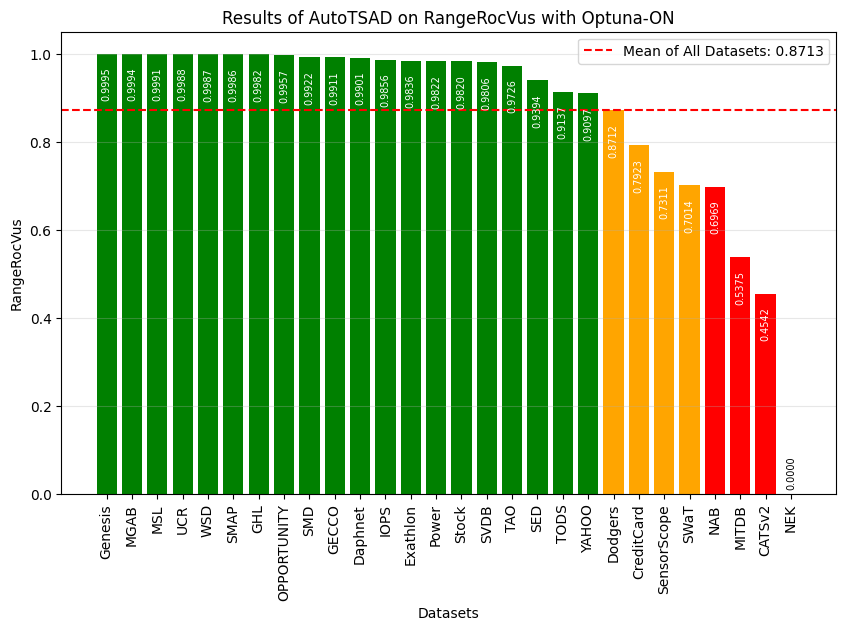
\includegraphics[width=1\linewidth]{Figures/v2_optuna-on_VUS.png}
    \caption{Συγκριτικά αποτελέσματα αλγορίθμων IForest - POLY - MP στην μετρική ROC-VUS.}
    \label{figure:tsad-vus-on}
\end{figure}

Από τους αλγορίθμους που εκτελέστηκαν από το \emph{TSB-UAD}, μπορούμε στο σχήμα \ref{figure:tsad-vus-compare} να παρατηρήσουμε την απόδοσή τους σε κάθε dataset μεμονωμένα, όπως επίσης και συγκριτικά πως τα πήγαν όλοι μαζί. Στο πάνω αριστερά σχήμα βλέπουμε την απόδοση του \emph{Iforest}, ο οποίοις φαίνεται ότι στα περισσότερα αποτελέσματα πέτυχε μία ικανοποιητική ανίχνευση ανωμαλιών, με χαμηλότερα αποτελέσματα να έχει πετύχει στα dataset \emph{WSD και Power}.
Αντίστοιχα πάνω δεξιά βλεόυμε την απόδοση του αλγορίθμου \emph{POLY}, ο οποίος έχει εμφανώς χειρότερα αποτελέσματα από τον \emph{IForest}, και σε 2 dataset, στα \emph{NEK} και \emph{UCR} έχει πετύχει απόδση μικρότερη του $20\%$.
Έπειτα, στο κάτω αριστερά σχήμα βλέπουμε τα αποτελέσματα του αλγορίθμου \emph{MP}, ο οποίος πάλι φαίνεται να έχει χειρότερα αποτελέσματα από τον \emph{IForest}, ενώ και αυτός έχει απόδοση μικρότερη του $20\%$ σε 2 dataset, διαφορετικά από τον αλγόριθμο \emph{POLY}, στα \emph{IOPS} και \emph{YAHOO}.
Τέλος στο κάτω δεξιά σχήμα, μπορούμε να δούμε συγκεντρωτικά τις αποδόσεις μεταξύ των αλγορίθμων που έτρεξαν μέσω του \emph{TSB-UAD}. 

\begin{figure}[h]
    \centering
    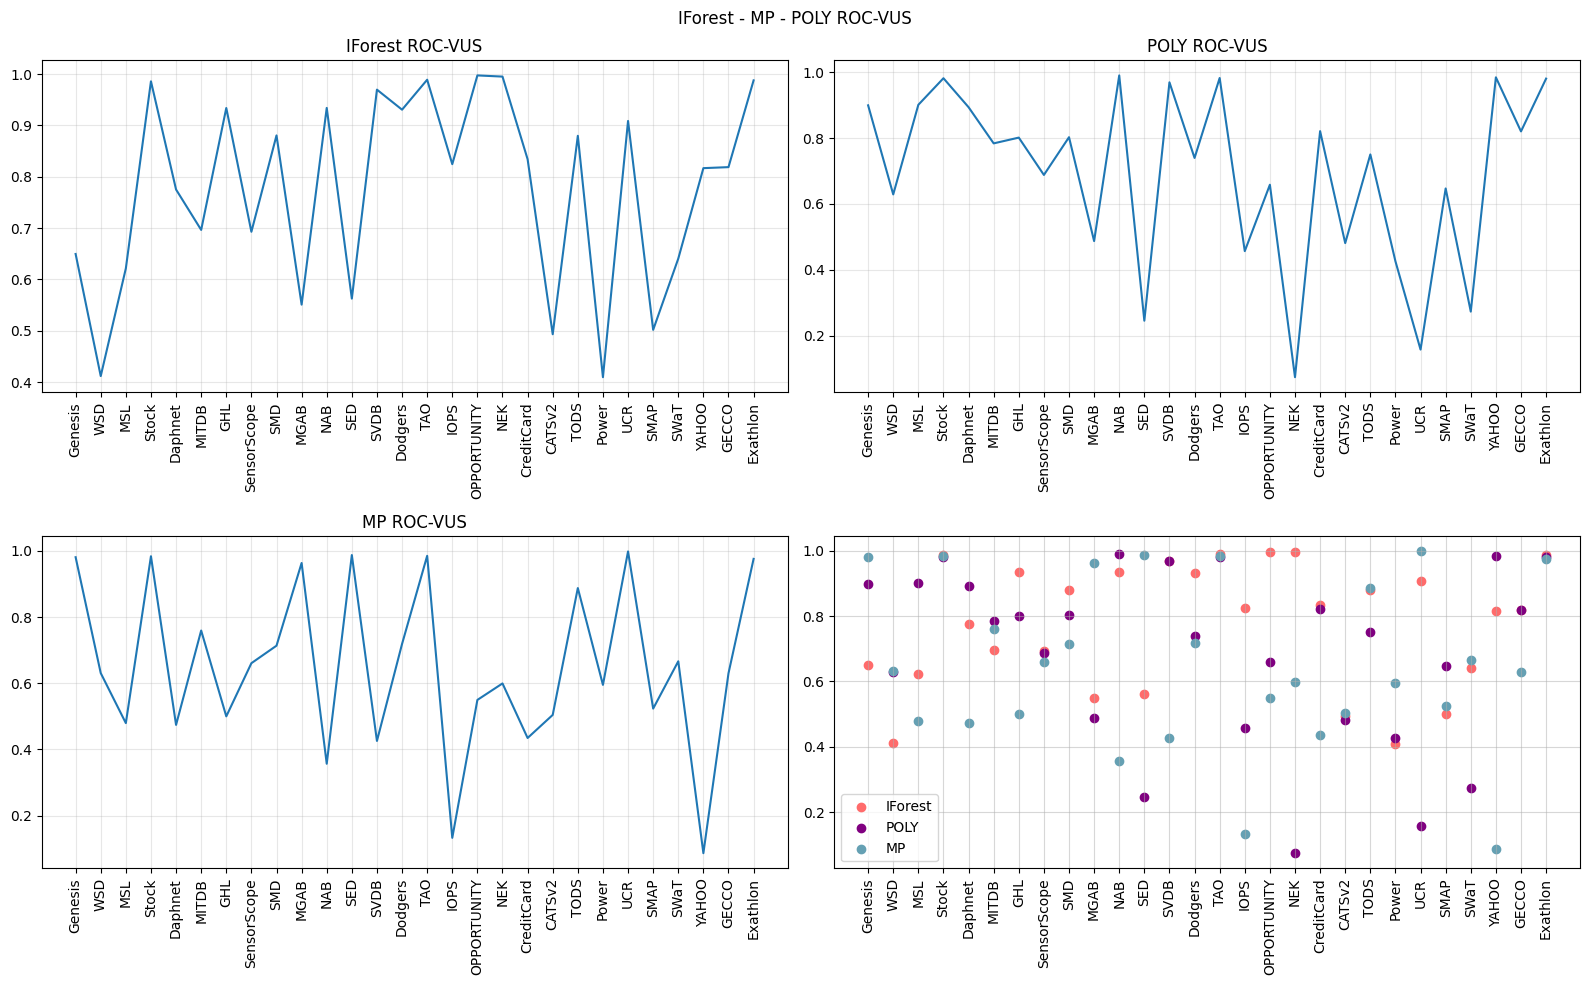
\includegraphics[width=1\linewidth]{Figures/v2_optuna-on_tsb-vus-compare.png}
    \caption{Αποτελέσματα χρήσης Optuna σε φθίνουσα σειρά.}
    \label{figure:tsad-vus-compare}
\end{figure}

Ιδιαίτερο ενδιαφέρον έχει όταν συγκρίνουμε όλα τα αποτελέσματα μεταξύ τους, δηλαδή του \emph{Auto-TSAD} και των αλγορίθμων του \emph{TSB-UAD}.Συγκριτκά τα αποτελέσματα του νικητήριου αλγορίθμου ανά dataset φαίνονται στον Πίνακα \ref{tab:winners}. Όπως φαίνεται και στο \ref{figure:vus-comparison-between-all}, θα περίμενε κανείς το \emph{Auto-TSAD}  να τα έχει πάει καλύτερα σε όλα τα dataset. Κάτι τέτοιο όμως δεν είναι αληθές και βλέπουμε ότι έχει καταφέρει να φέρει καλύτερα αποτελέσματα, μόνο στο $57,16\%$ των περιπτώσεων, γεγονός το οποίο είναι ιδιαίτερα χαμηλό αν αναλογιστεί κανείς το χρονικό κόστος. Η σημαντικότερη όμως παρατήρηση είναι, πως ακόμα και αν δεν κατάφερε να υπερτερήσει σε όλες τις περιπτώσεις, ήταν πολύ κοντά στην μέγιστη τιμή ανωμαλιών που ανιχτέυτηκε από τις άλλες τεχνικές.

\begin{table}
\centering
\caption{Νικητήριος Αλγόριθμος ανά Dataset}
\label{tab:winners}
\begin{tabular}{llc}
\toprule
 & Winner & Score \\
\midrule
Genesis & AutoTSAD & 0.9995 \\
WSD & AutoTSAD & 0.9987 \\
MSL & AutoTSAD & 0.9991 \\
Stock & IForest & 0.9860 \\
Daphnet & AutoTSAD & 0.9901 \\
MITDB & POLY & 0.7839 \\
GHL & AutoTSAD & 0.9982 \\
SensorScope & AutoTSAD & 0.7311 \\
SMD & AutoTSAD & 0.9922 \\
MGAB & AutoTSAD & 0.9994 \\
NAB & POLY & 0.9902 \\
SED & MP & 0.9873 \\
SVDB & AutoTSAD & 0.9806 \\
Dodgers & IForest & 0.9307 \\
TAO & IForest & 0.9891 \\
IOPS & AutoTSAD & 0.9856 \\
OPPORTUNITY & IForest & 0.9975 \\
NEK & IForest & 0.9953 \\
CreditCard & IForest & 0.8342 \\
CATSv2 & MP & 0.5044 \\
TODS & AutoTSAD & 0.9137 \\
Power & AutoTSAD & 0.9822 \\
UCR & AutoTSAD & 0.9988 \\
SMAP & AutoTSAD & 0.9986 \\
SWaT & AutoTSAD & 0.7014 \\
YAHOO & POLY & 0.9844 \\
GECCO & AutoTSAD & 0.9911 \\
Exathlon & IForest & 0.9879 \\
\bottomrule
\end{tabular}
\end{table}

\begin{figure}[h]
    \centering
    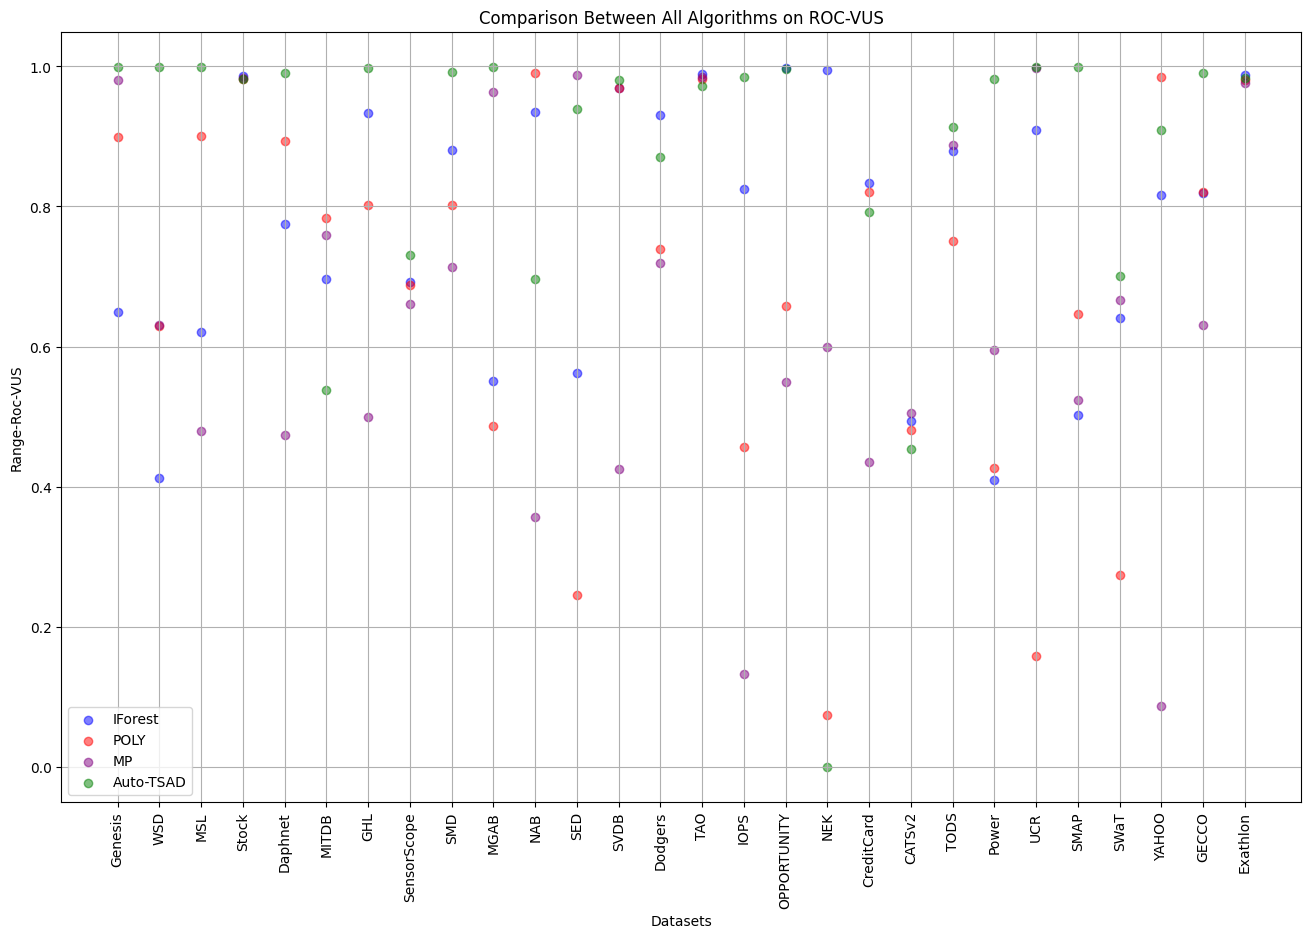
\includegraphics[width=1\linewidth]{Figures/vus-comparison-between-all.png}
    \caption{Σύγκριση μεταξύ όλων των τεχνικών.}
    \label{figure:vus-comparison-between-all}
\end{figure}

Πιο συγκερκιμένα και όπως φαίνεται και στο boxplot του σχήματος \ref{figure:more-comparisons}, το \emph{Auto-TSAD} έχει πολύ πιο σταθερή απόδοση σε σχέση με τους υπόλοιπους αλγορίθμους. Η διάμεσός του, η οποία δεν φαίνεται καθαρά, αγγίζει σχεδόν το $1.0$ και το κουτί του, είναι εξαιρετικά συμπιεσμένο προς τα πάνω. Ακολουθεί ο αλγόριθμος \emph{IForest} με καλύτερα αποτελέσματα από τους άλλους, ενώ ο \emph{POLY} και ο \emph{MP} έχουν σχεδόν παρόμοια συμπεριφορά.
Το barchart του σχήματος \ref{figure:more-comparisons} μας δείχνει ξεκάθαρα πως το \emph{Auto-TSAD} κυριαρχεί έναντι των άλλων μεθόδων με 16 νίκες, έναντι του \emph{IForest} με 8 νίκες και των \emph{POLY} και \emph{MP} με 3 και 2 νίκες αντιστοίχως.
Στο 3ο διάγραμμα του σχήματος \ref{figure:more-comparisons}, όποια κουκίδα βρίσκεται κάτω και δεξιά από την γραμμή $y=x$, σημαίνει ότι το \emph{Auto-TSAD} ξεπέρασε τον αντίστοιχο αλγόριθμο. Παρατηρήτε μία συγκέντρωση κουκκίδων, στην τέρμα δεξιά πλευρά, γεγονός το οποίο μας δείχνει πως όταν το \emph{Auto-TSAD} κατάφερε να πιάσει σχεδόν $100\%$ των ανωμαλιών, οι άλλοι αλγόριθμοι αποτύγχαναν αρκετές φορές. 

\begin{figure}[h]
    \centering
    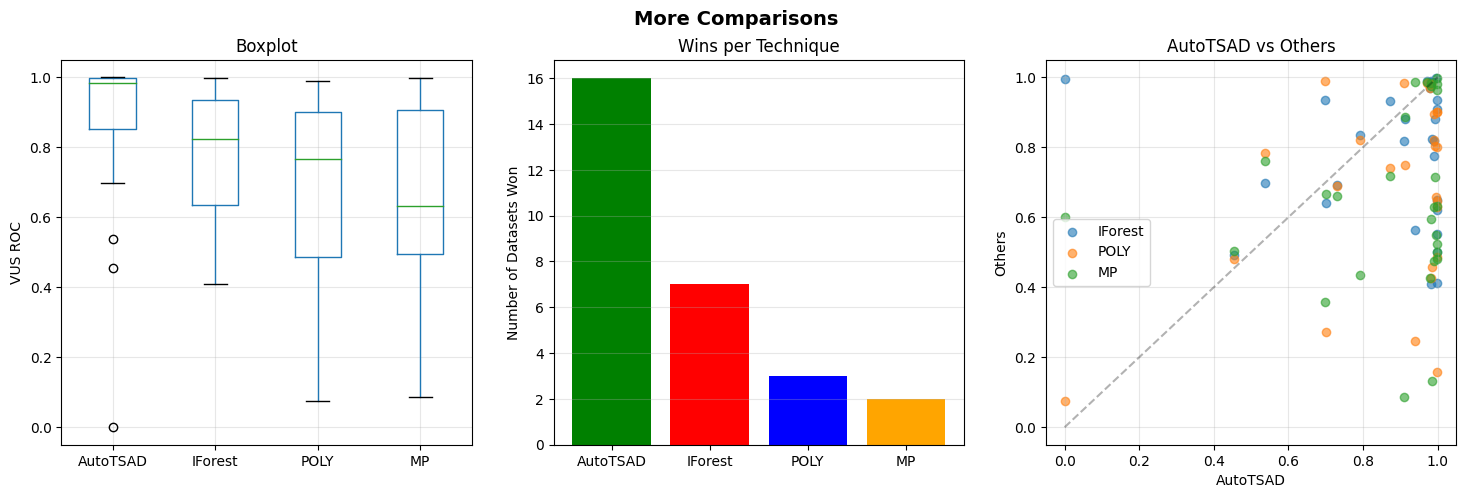
\includegraphics[width=1\linewidth]{Figures/v2_optuna-on_more_comparisons.png}
    \caption{Σύγκριση μεταξύ όλων των τεχνικών.}
    \label{figure:more-comparisons}
\end{figure}

Φτάνουμε λοιπόν στο συμπέρασμα πως υπάρχει ένα ξεκάθαρο αντιστάθισμα μεταξύ υπολογιστικού κόστους και ακρίβειας. Αν και η εκτέλεση μεμονωμένων αλγόριθμων απαιτεί μόνο μερικά δευτερόλεπτα με προκαθορισμένες υπερπαραμέτρους, η απόδοσή τους είναι εξαιρετικά ασταθής. Σε αντίθεση, οι τεχνικές βελτιστοποίησης του \emph{Auto-TSAD} αν και εκτοξεύουν το χρόνο εκτέλεσης σε τάξης αρκετών ωρών ή ακόμα και ημερών, εξασφαλίζουν σταθερότητα και ανωτερότητα στην εύρεση ενωμαλιών, εκτός μεμονωμένων περιπτώσεων.

\subsubsection{Συγκριτικά αποτελέσματα με Optuna-OFF}
Όπως έχουμε αναφέρει και στην αρχή του κεφαλαίου, χωρίς την μηχανή βελτιστοποίησης \emph{Optuna}, το \emph{Auto-TSAD} μπόρεσε να υπολογίσει αποτελέσματα μόνο στο $31,2\%$ των περιπτώσεων, ποσοστό αρκετά χαμηλό .
Στο σχήμα \ref{figure:roc-vus_optuna_off_v2} παρατηρούμε ότι οι τιμές της ROC-VUS διαφέρουν αρκετά σχετικά με το αν συμπεριλάβουμε τις αποτυχημένες προσπάθειες ή όχι. Συγκεκριμένα:
\begin{itemize}
    \item \strong{Με} συμπερίληψη των αποτυχημένων προσπαθειών, βλέπουμε ότι οι τιμές της ROV-VUS επειρεάζονται αρκετά από τις αποτυχίες και περιορίζονται στο διάστημα $[0,0.4]$. Επίσης η διάμεσος είναι $0.33$ και η τυπική απόκληση $0.41$.
    \item \strong{Χωρίς} συμπερίληψη αποτυχημένων προσπαθειών, η εικόνα αλλάζει δραματικά, η ελάχιστη τιμή είναι περίπου $0.42$, η μέγιστη αγγίζει το απόλυτο, ενώ υπάρχει μία συγκέντρωση τιμών στο διάστημα $[0.73, 0.96]$. Η διάμεσος είναι $0.84$ ενώ η τυπική απόκλιση είναι $0.11$.   
\end{itemize}
Παρατηρούμε λοιπόν, πως υπάρχει σημαντική διαφορά των αποτελεσμάτων, αν δεν συμπεριλάβουμε τα αποτελέσματα των αποτυχημένων προσπαθειών. 

\begin{figure}[h]
    \centering
    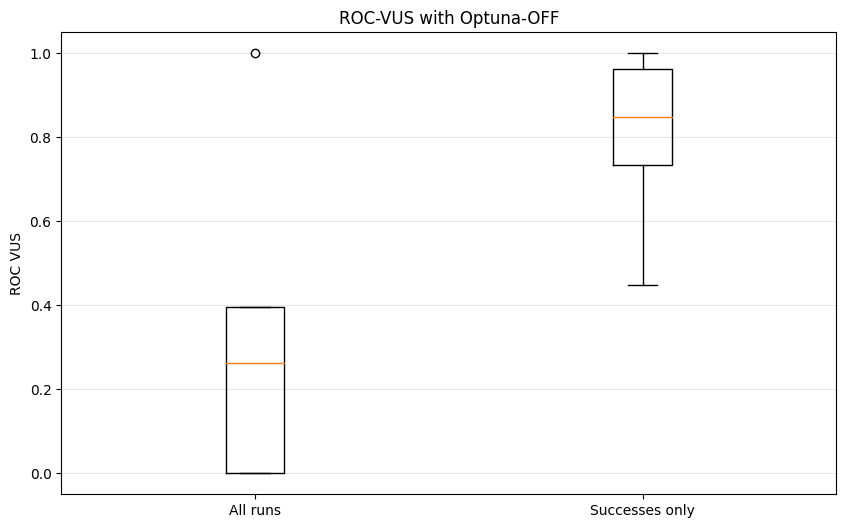
\includegraphics[width=0.8\linewidth]{Figures/roc-vus_optuna_off_v2.png}
    \caption{Αποτελέσματα Auto-TSAD με Optuna-OFF στο v2\_public dataset.}
    \label{figure:roc-vus_optuna_off_v2}
\end{figure}

Στο σχήμα \ref{figure:comparison_Between_Auto-TSAD_WO_Optuna_and_TSB-UAD_algorithms}, στο οποίο συγκρίνουμε την απόδοση του \emph{Auto-TSAD} χωρίς \emph{Optuna} με τους αλγορίθμους το \emph{TSB-UAD}, βλέπουμε πως, όταν ο \emph{Auto-TSAD} καταφέρνει να δώσει αποτέλεσμα, είναι αρκετά πιο αποτελεσματικούς από τους υπόλοιπους αλγορίθμους. Αν αντιθέτως συγκρίνουμε τα στατιστικά του συνυπολογίζοντας και τις αποτυχίες του, τότε οι απλοί αλγόριθμοι υπερτερούν αρκετά. Το μεγάλο πλεονέκτημα των αλγορίθμων του \emph{TSB-UAD}, είναι πως πάντα θα καταφέρουν να υπολογίσουν ένα μέρος των ανωμαλιών της χρονοσειράς που εξετάζουν, ακόμα και αν το αποτέλεσμα τους δεν είναι ικανοποιητικό. 
\begin{figure}[h]
    \centering
    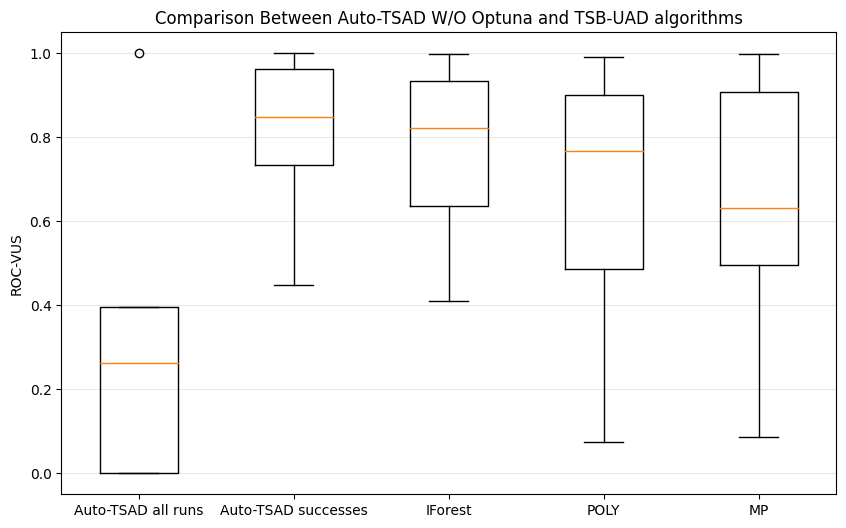
\includegraphics[width=0.8\linewidth]{Figures/Comparison_Between_Auto-TSAD_WO_Optuna_and_TSB-UAD_algorithms.png}
    \caption{Σύγκριση αποτελεσμάτων μεταξύ Auto-TSAD χωρίς Optuna και TSB-UAD.}
    \label{figure:comparison_Between_Auto-TSAD_WO_Optuna_and_TSB-UAD_algorithms}
\end{figure}

\textcolor{red}{ΕΡΩΤΗΜΑ ΠΡΟΣ Κ.ΓΟΥΝΑΡΗ. ΑΝ ΘΕΛΕΤΕ ΜΠΟΡΩ ΚΑΙ ΕΔΩ ΝΑ ΚΑΝΩ ΑΝΑΛΥΣΗ ΑΝΑ DATASET, ΚΑΙ ΟΧΙ ΣΥΓΚΕΝΤΡΩΤΙΚΑ.}
\section{Artificial Dataset}
\textcolor{red}{ΠΡΟΣ Κ.ΓΟΥΝΑΡΗ. ΕΔΩ ΘΑ ΕΧΩ ΤΗΝ ΙΔΙΑ ΑΝΑΛΥΣΗ ΟΠΩΣ ΣΤΟ PUBLIC DATASET, ΑΠΛΑ ΕΠΕΙΔΗ ΤO ARTIFICIAL ΔΕΝ ΧΩΡΊΖΕΙ ΣΕ ΔΙΑΦΟΡΕΤΙΚΟΥ ΤΥΠΟΥ ΔΕΔΟΜΕΝΩΝ Η ΑΝΑΛΥΣΗ ΘΑ ΕΙΝΑΙ ΠΙΟ ΣΥΝΤΟΜΗ}
\section{ΚΕΡΔΟΣ ΑΝΑ ΧΡΟΝΟ}
\textcolor{red}{ΠΡΟΣ Κ.ΓΟΥΝΑΡΗ. ΕΔΩ ΘΑ ΒΑΛΩ ΑΥΤΟ ΠΟΥ ΜΕ ΕΙΠΑΤΕ, ΟΠΟΥ ΘΑ ΠΟΣΟ ΚΕΡΔΙΖΩ ΣΤΗΝ ROC VUS // ΜΟΝΑΔΕΣ ΧΡΟΝΟΥ}
%\include{Chapters/Chapter4} 
%\include{Chapters/Chapter5} 

%----------------------------------------------------------------------------------------
%	THESIS CONTENT - APPENDICES
%----------------------------------------------------------------------------------------

\appendix % Cue to tell LaTeX that the following "chapters" are Appendices

% Include the appendices of the thesis as separate files from the Appendices folder
% Uncomment the lines as you write the Appendices

\include{Appendices/AppendixA}
%\include{Appendices/AppendixB}
%\include{Appendices/AppendixC}

%----------------------------------------------------------------------------------------
%	BIBLIOGRAPHY
%----------------------------------------------------------------------------------------

\printbibliography[heading=bibintoc]

%----------------------------------------------------------------------------------------

\end{document}  
